%%%%%%%% ICML 2026 EXAMPLE LATEX SUBMISSION FILE %%%%%%%%%%%%%%%%%

\documentclass{article}

% Recommended, but optional, packages for figures and better typesetting:
\usepackage{microtype}
\usepackage{graphicx}
\usepackage{subcaption}
\usepackage{booktabs} % for professional tables

\usepackage{enumitem}
\usepackage{tcolorbox}
\tcbuselibrary{listings, skins, breakable}
\usepackage{xcolor}

% 自定义一个灰黑风格的 prompt box
\newtcolorbox{promptbox}[2][]{enhanced, breakable,
  colback=gray!10, colframe=black!60,
  coltitle=white, fonttitle=\bfseries,
  title=#2, #1}
% hyperref makes hyperlinks in the resulting PDF.
% If your build breaks (sometimes temporarily if a hyperlink spans a page)
% please comment out the following usepackage line and replace
% \usepackage{icml2026} with \usepackage[nohyperref]{icml2026} above.
\usepackage{hyperref}


% Attempt to make hyperref and algorithmic work together better:
\newcommand{\theHalgorithm}{\arabic{algorithm}}

% Use the following line for the initial blind version submitted for review:
\usepackage[preprint]{icml2026}

% For preprint, use
% \usepackage[preprint]{icml2026}

% If accepted, instead use the following line for the camera-ready submission:
% \usepackage[accepted]{icml2026}

\usepackage{amsmath}
\usepackage{amssymb}
\usepackage{mathtools}
\usepackage{amsthm}

\usepackage{multirow}
\usepackage{colortbl}
\usepackage{xcolor}
\definecolor{graybg}{gray}{0.95} % 定义淡淡的灰色背景
\newcommand{\cgap}[1]{\scriptsize{\color{teal}(+#1)}}
% if you use cleveref..
\usepackage[capitalize,noabbrev]{cleveref}

\usepackage{enumitem}

%%%%%%%%%%%%%%%%%%%%%%%%%%%%%%%%
% THEOREMS
%%%%%%%%%%%%%%%%%%%%%%%%%%%%%%%%
\theoremstyle{plain}
\newtheorem{theorem}{Theorem}[section]
\newtheorem{proposition}[theorem]{Proposition}
\newtheorem{lemma}[theorem]{Lemma}
\newtheorem{corollary}[theorem]{Corollary}
\theoremstyle{definition}
\newtheorem{definition}[theorem]{Definition}
\newtheorem{assumption}[theorem]{Assumption}
\theoremstyle{remark}
\newtheorem{remark}[theorem]{Remark}

% Todonotes is useful during development; simply uncomment the next line
%    and comment out the line below the next line to turn off comments
%\usepackage[disable,textsize=tiny]{todonotes}
\usepackage[disable,textsize=tiny]{todonotes}

% The \icmltitle you define below is probably too long as a header.
% Therefore, a short form for the running title is supplied here:
%\icmltitlerunning{Submission and Formatting Instructions for ICML 2026}
\icmltitlerunning{Auditing Multi-Agent LLM Reasoning Trees}
\icmlsetsymbol{equal}{*}
\begin{document}

\twocolumn[
  % \icmltitle{Truth is Not a Vote: Dismantling Confabulation Consensus in  \\ Multi-Agent LLM Systems via Reasoning Tree Auditing}
  \icmltitle{Auditing Multi-Agent LLM Reasoning Trees \\Outperforms Majority Vote and LLM-as-Judge}

  % It is OKAY to include author information, even for blind submissions: the
  % style file will automatically remove it for you unless you've provided
  % the [accepted] option to the icml2026 package.

  % List of affiliations: The first argument should be a (short) identifier you
  % will use later to specify author affiliations Academic affiliations
  % should list Department, University, City, Region, Country Industry
  % affiliations should list Company, City, Region, Country

  % You can specify symbols, otherwise they are numbered in order. Ideally, you
  % should not use this facility. Affiliations will be numbered in order of
  % appearance and this is the preferred way.
  
    \begin{icmlauthorlist}
      \icmlauthor{Wei Yang}{equal,usc}
      \icmlauthor{Shixuan Li}{equal,usc}
      \icmlauthor{Heng Ping}{usc}
      \icmlauthor{Peiyu Zhang}{usc}
      \icmlauthor{Paul Bogdan}{usc}
      \icmlauthor{Jesse Thomason}{usc}
    \end{icmlauthorlist}
    \icmlaffiliation{usc}{University of Southern California, Los Angeles, CA, USA}
  %\icmlcorrespondingauthor{Firstname1 Lastname1}{first1.last1@xxx.edu}
  %\icmlcorrespondingauthor{Firstname2 Lastname2}{first2.last2@www.uk}

   \icmlcorrespondingauthor{Wei Yang}{wyang930@usc.edu}
   \icmlcorrespondingauthor{Shixuan Li}{sli97750@usc.edu}
   \icmlcorrespondingauthor{Jesse Thomason}{jessetho@usc.edu}

    
  % You may provide any keywords that you find helpful for describing your
  % paper; these are used to populate the "keywords" metadata in the PDF but
  % will not be shown in the document
  
  %\icmlkeywords{Machine Learning, ICML}
  %\printAffiliationsAndNotice{\icmlEqualContribution}
    
  \vskip 0.3in
]
\printAffiliationsAndNotice{\icmlEqualContribution}
% this must go after the closing bracket ] following \twocolumn[ ...

% This command actually creates the footnote in the first column listing the
% affiliations and the copyright notice. The command takes one argument, which
% is text to display at the start of the footnote. The \icmlEqualContribution
% command is standard text for equal contribution. Remove it (just {}) if you
% do not need this facility.

% Use ONE of the following lines. DO NOT remove the command.
% If you have no special notice, KEEP empty braces:
%\printAffiliationsAndNotice{}  % no special notice (required even if empty)
% Or, if applicable, use the standard equal contribution text:
% \printAffiliationsAndNotice{\icmlEqualContribution}

\begin{abstract}
% Multi-agent systems (MAS) can substantially extend the reasoning capacity of large language models (LLMs), yet most frameworks still aggregate agent outputs with majority voting. This heuristic discards the evidential structure of reasoning traces and is brittle under confabulation consensus, where agents share correlated biases and converge on the same incorrect rationale. To address this epistemic failure, we introduce \textbf{AgentAuditor}, an agentic structure-adaptive non-voting auditor, which replaces voting with a path search over a Reasoning Tree that explicitly represents agreements and divergences among agent traces. AgentAuditor resolves conflicts using a Structure-Adaptive Auditor that compares branches only at Critical Divergence Points, turning global adjudication into efficient localized verification. To reduce the Auditor's tendency to follow majority support, we further propose Anti-Consensus Preference Optimization (ACPO), which trains the adjudicator on majority-failure cases and rewards evidence-based minority selections over popular errors. Across diverse MAS settings, AgentAuditor consistently escapes the consensus trap and yields up to 5\% absolute improvement over majority voting.
Multi-agent systems (MAS) can substantially extend the reasoning capacity of large language models (LLMs), yet most frameworks still aggregate agent outputs with majority voting. This heuristic discards the evidential structure of reasoning traces and is brittle under the confabulation consensus, where agents share correlated biases and converge on the same incorrect rationale. 
We introduce \textbf{AgentAuditor}, which replaces voting with a path search over a Reasoning Tree that explicitly represents agreements and divergences among agent traces. 
AgentAuditor resolves conflicts by comparing reasoning branches at critical divergence points, turning global adjudication into efficient, localized verification. 
We further propose Anti-Consensus Preference Optimization (ACPO), which trains the adjudicator on majority-failure cases and rewards evidence-based minority selections over popular errors. 
AgentAuditor is agnostic to MAS setting, and we find across 5 popular settings that it yields up to 5\% absolute accuracy improvement over a majority vote, and up to 3\% over using LLM-as-Judge.
\end{abstract}

\section{Introduction}

Multi-agent systems (MAS) built on large language models (LLMs) are rapidly becoming a dominant paradigm for complex problem solving~\cite{zhang2024proagent,qiao2024autoact,han2025joyagents,ye2024domain,ping2025hdlcore,chang2025survey}. 
By orchestrating multiple LLM agents via debate and critique~\citep{du2023improving,liu2024groupdebate,ping2025verimoa}, dynamic computation graphs~\cite{zhang2024aflow,han2025joyagents}, and structured communication topologies~\citep{gabriel2024advancing,li2025adaptive,yang2025maestro}, modern MAS can substantially expand reasoning depth beyond a single-pass generation~\cite{park2023generative, zhu2025lamarl,chen2026self}.
However, this progress exposes a striking bottleneck. Despite increasingly sophisticated generation and interaction, the final decision rule is often reduced to majority voting~\cite{hong2023metagpt,ning2023skeleton}. 
This creates a mismatch where rich multi-agent reasoning is ultimately compressed into a crude final rule.~\cite{xie2023self,zhang2024self}. 



\begin{figure}[t]
    \centering
    
\includegraphics[width=\linewidth]{figures/intro.pdf}
    \caption{\textbf{Majority voting vs.\ AgentAuditor.}
\emph{Left:} Majority voting can follow the herd into a dominant but wrong consensus.
\emph{Right:} AgentAuditor audits localized branch evidence on a reasoning tree to reliably select the correct minority answer. This contrasts frequency-based selection with evidence-based adjudication under confabulation consensus.}
    \label{fig:intro}
\end{figure}


Majority voting is appealing for its simplicity, yet it rests on an epistemic assumption that breaks in LLM collectives~\cite{jiang2023llm,qiao2024autoact,yan2024mirror}.
While computationally convenient, it inherits the Condorcet Jury Theorem~\cite{austen1996information} assumption that agents' errors are independent.
This assumption collapses in practice because LLM agents are not epistemically independent. They often share similar pre-training manifolds and alignment biases, and they can also become anchored to the same misleading cues in the prompt. As a result, groups can fall into \textit{confabulation consensus}, where agents reinforce each other's hallucinated rationale rather than correcting it~\cite{mahaut2024factual,coeckelbergh2025llms}. These errors are therefore not random noise. They often repeat the same incorrect intermediate claims, making frequency a poor proxy for validity.
Voting further amplifies this failure mode by collapsing rich reasoning traces into context-free tallies, discarding the evidential process required for verification~\citep{wang2023unleashing,chen2024routerdc}. Consequently, MAS may converge with high confidence on an incorrect answer because the same flawed argument is repeated, even when a minority branch offers stronger evidence~\citep{pitre2025consensagent,bai2024confidencecal}.

To break this confabulation consensus, the system must transition from statistical aggregation to substantive evaluation~\citep{zhou2025reso,wang2024self,xu2025scalable,li2024verco,adewumi2024limitations}. A straightforward alternative is to adopt an LLM-as-a-Judge, yet naive judging is insufficient because it is both computationally inefficient and prone to sycophancy bias. Structurally, asking the judge to read the full context of every agent's trace to spot errors scales prohibitively with the number of agents and the length of reasoning. Long prefixes and late-stage hallucinations further dilute attention, making it hard for a judge to isolate the true point of disagreement. 
More critically, judge models themselves can be biased by majority cues in the same way as the agents.
When faced with a majority-minority split such as ``3 vs.\ 1'', standard LLMs often show strong conformity and default to the majority view, even when the minority is better supported. A robust adjudicator should concentrate computation on decision-critical disagreements while remaining agnostic to popularity signals, so majority support does not override evidence.


To bridge this gap, we propose \textbf{AgentAuditor}, an agentic structure-adaptive non-voting auditing framework. Instead of treating consensus as a headcount, AgentAuditor searches a reasoning structure for the most justified path. As shown in Figure\ref{fig:intro}, AgentAuditor can select the correct answer in situations where there are only a few correct answers. \textbf{AgentAuditor} organizes collective reasoning traces into a Reasoning Tree, where agreements form shared prefixes and disagreements become explicit topological bifurcations. 
This structure supports a Structure-Adaptive Auditor that performs differential diagnosis only at Critical Divergence Points (CDPs), converting global evaluation into localized pairwise comparisons. 
By focusing the audit on the immediate logical split, AgentAuditor makes verification local. At a divergence, it is often easier to decide which branch is better supported than to reconstruct the full solution.
Crucially, we further train the Auditor with \textbf{Anti-Consensus Preference Optimization (ACPO)}, an alignment strategy constructed from historical majority-failure cases that explicitly penalizes popular-but-wrong decisions and rewards minority-but-correct reasoning. 
%ACPO thus pushes the Auditor to prioritize evidence over majority support, targeting the consensus trap.


In summary, we highlight the main contributions of this work as follows:
\begin{itemize}[noitemsep,nosep]
    \item We propose AgentAuditor, replacing multi-agent majority voting with a reasoning tree structure that enables effective context-aware evidence auditing.
    \item We introduce ACPO, a training strategy that immunizes the Auditor against sycophancy bias by optimizing for minority-truth.
    \item Extensive experiments across MAS frameworks show that AgentAuditor consistently identifies correct minority answers, outperforming majority voting baselines.
\end{itemize}



\section{Related Work}
%% Short Version
\subsection{LLM-based Multi-Agent Reasoning}
LLM-based multi-agent systems (MAS) ~\cite{yang2025toward,qiao2024autoact,yang2025learning} have become a common strategy for improving complex reasoning by enabling distributed exploration, critique, and coordination~\cite{hong2023metagpt,chen2023agentverse,wu2024autogen,zhang2024aflow,ning2023skeleton}. 
Prior work spans (i) pre-structured interaction protocols such as debate-style exchanges or fixed topologies that regulate information flow and verification~\cite{du2023improving,liu2024groupdebate}, and (ii) self-organizing paradigms that dynamically route, prune, or evolve collaboration graphs for efficiency and diversity~\cite{hu2024automated,zhuge2024gptswarm,zhang2024aflow}. 
While these methods primarily optimize how agents interact, they often leave the final adjudication rule comparatively under-specified, which can make the collective outcome vulnerable when agent errors are correlated~\citep{wei2025lero,jiang2025qllm,alsadat2024multi,lin2025speaking}.
A more comprehensive discussion is provided in Appendix.~\ref{app:relatedwork_part1}.

%% Short Version
\subsection{Evaluation and Adjudication in MAS}
A central challenge in multi-agent reasoning is converting diverse traces into a reliable final decision. 
Many systems still rely on majority voting or simple ensembling heuristics~\cite{chan2023chateval,chen2024llmarena,wei2025lero}, which can fail under correlated mistakes. 
These approaches often treat each trace as an indivisible unit, leaving limited support for localized, evidence-conditioned comparison across disagreements.
To improve reliability, recent work explores referee agents, debate adjudication, and peer-review style evaluation of reasoning trajectories~\cite{abdelnabi2023llm,du2023improving,wang2025mars}. 
In parallel, LLM evaluation and verification studies develop reward modeling and reflective self-critique mechanisms~\cite{kwon2023reward,xie2023self,zhang2024self,yan2024mirror}, but these are typically designed for single-agent settings rather than structure-aware multi-agent adjudication~\cite{lambert2024rewardbench,setlur2024rewarding}. 
A fuller related-work taxonomy and comparisons appear in Appendix.~\ref{app:relatedwork_part2}.


%\subsection{LLM-based Multi-Agent Collaboration for Reasoning}
%Recent advances in large language models (LLMs) have fueled multi-agent systems (MAS) that extend single-model reasoning via interaction and cross-checking~\cite{wu2024autogen,motwani2024malt,ishibashi2024self,yan2025beyond,dai2025multi}. Representative frameworks show that distributed exploration and mutual critique can improve reasoning quality~\cite{hong2023metagpt,chen2023agentverse,jiang2023llm,ning2023skeleton,qiao2024autoact,pan2024agentcoord}. Existing methods can be roughly grouped into two styles. Prestructured collaboration uses fixed topologies such as chains, trees, debate graphs to organize discussion and verification~\cite{du2023improving,liu2024groupdebate,qian2024scaling}, offering coherent interaction but limited adaptivity. Self-organizing approaches instead learn or evolve communication graphs through routing, pruning, or evolutionary coordination, as in DyLan, GPTSwarm, and AFLOW~\cite{hu2024automated,shang2024agentsquare,zhang2024cut,zhuge2024gptswarm,zhang2024aflow}. Despite progress in coordination efficiency and diversity~\citep{wan2025rema,peiyuan2024agile,feng2024large}, most work emphasizes how agents communicate rather than how to adjudicate conflicting reasoning. As a result, collectives remain exposed to correlated failures and unverified consensus, where agreement can be driven by shared biases instead of evidence~\citep{wei2025lero,jiang2025qllm,alsadat2024multi,lin2025speaking}. 

%\subsection{Evaluation and Adjudication in Multi-Agent Reasoning}
%While multi-agent coordination can broaden exploration, ensuring the correctness of the collective output remains difficult. Many systems still rely on majority voting or rule-based ensembling~\cite{chan2023chateval,chen2024llmarena,wei2025lero}, implicitly treating agreement as a proxy for truth. However, when agents share similar training distributions, their errors can be correlated, making the majority confidently converge to a plausible but wrong answer, a failure sometimes characterized as the ``tyranny of the majority''~\cite{du2023improving,liu2024groupdebate}. To improve reliability, recent work introduces referee or reviewer agents that assess peers' reasoning trajectories~\cite{abdelnabi2023llm,du2023improving,zhang2024cut}. Debate-style protocols surface competing arguments before a judge selects a winner, while self-consistency and peer-review variants aggregate explanations rather than only final answers~\cite{chen2023universal,xu2023towards,wang2025mars}. In parallel, research on LLM evaluation and verification studies automated validation via reward modeling~\cite{kwon2023reward,lambert2024rewardbench,setlur2024rewarding} and reflective self-evaluation~\cite{xie2023self,zhang2024self,yan2024mirror}. %Nonetheless, many of these methods rely on heuristic templates or single-agent reflection, and do not directly address \emph{distributed} adjudication that is both evidence-grounded and robust to majority bias.







\begin{figure*}[t]
    \centering
    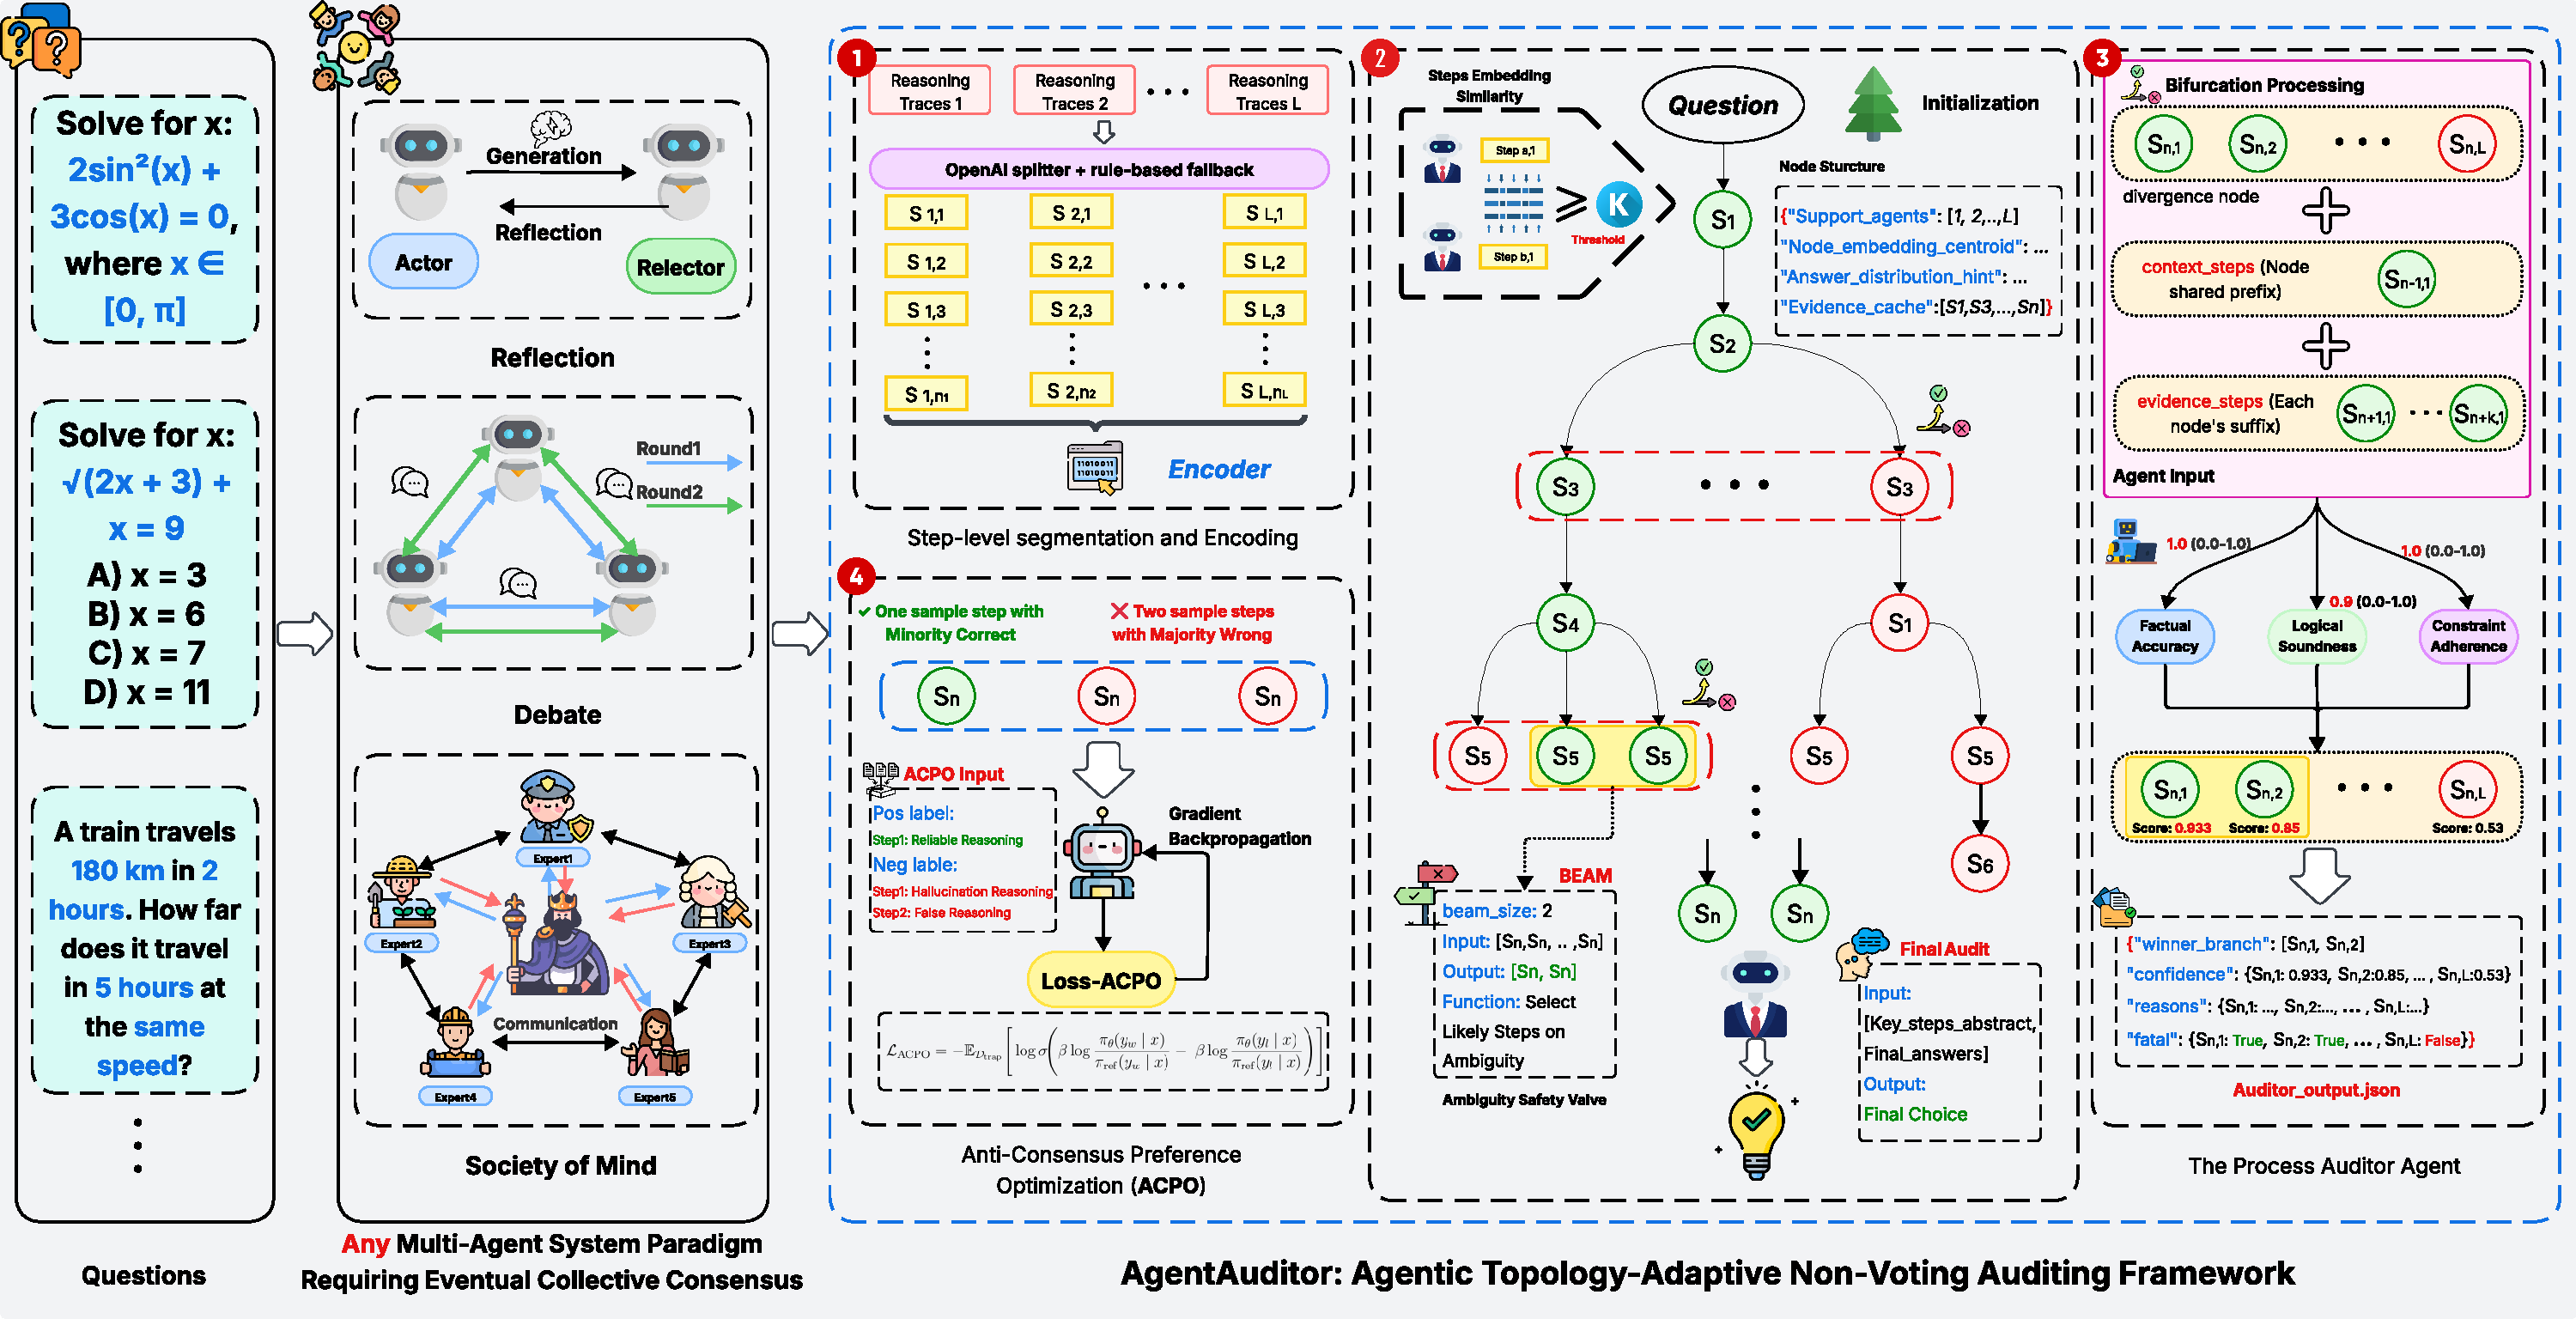
\includegraphics[width=\textwidth]{figures/overall_arch.pdf}
    \caption{\textbf{Overall architecture of AgentAuditor framework.}
Given a multi-agent slate of reasoning traces, AgentAuditor performs structural semantic deduplication to construct a compact \textbf{Reasoning Tree} of distinct hypotheses.
It then audits only decision-critical \textbf{Divergence Points} by comparing localized branch evidence, selecting the winning hypothesis and propagating its answer as the final aggregation.
For learnable auditing, we train the Auditor with \textit{Anti-Consensus Preference Optimization} on consensus-trap instances.}
    \label{fig:architecture}
\end{figure*}




 \section{Problem Formulation}
\label{sec:formal_setup}


\paragraph{Setting.}
Given a query $q$ with ground-truth answer $y^\star$, a multi-agent system runs $N$ agents and produces outputs
$\mathcal{O}=\{o_1,\ldots,o_N\}$, where each $o_i$ contains a reasoning trace and a final answer $\hat{y}(o_i)$.
We view each $o_i$ as inducing a semantic hypothesis about how to answer $q$ (e.g., a reasoning branch), together with the evidence it cites.
An \emph{aggregator} maps the set of agent outputs to a single prediction, i.e., $\hat{y}=f(\mathcal{O}, q)$, where a standard and widely used baseline is \emph{majority voting} over the agents’ final answers.

\paragraph{Failure mode: confabulation consensus.}
LLM-based MAS often exhibits \emph{confabulation consensus}, where many agents generate semantically similar rationales and converge to the same
incorrect conclusion. We capture this as a mismatch between quantity and validity.
Let $\mathcal{B}=\{B_1,\ldots,B_K\}$ denote the set of \emph{distinct semantic hypotheses} underlying $\mathcal{O}$ (e.g., distinct reasoning
branches), where redundancy implies $K \ll N$.
Let $m_k$ be the \emph{multiplicity} of hypothesis $B_k$, i.e., the number of agents whose outputs support $B_k$.
Under confabulation consensus, an erroneous hypothesis can have $m_{\mathrm{err}} \gg m_{\mathrm{cor}}$ even when a correct hypothesis exists, so frequency is not a reliable proxy. % for correctness.


\paragraph{Objective.}
We seek an aggregator $\hat{y}=f(\mathcal{O}, q)$ that is \emph{robust to multiplicity} (not inherently favoring hypotheses with larger $m_k$) yet \emph{sensitive to evidence} (recovering $y^\star$ when a correct hypothesis is present but outnumbered). AgentAuditor operationalizes this objective by (i) semantically deduplicating $\mathcal{O}$ into a compact tree over $\mathcal{B}$, and (ii) auditing only at decision-critical divergence points, replacing frequency-driven selection with evidence-based discrimination under structured multi-agent redundancy.


\paragraph{Theoretical formulation.}
We provide a lightweight theoretical analysis in Appendix~\ref{app:toy_analysis} that formalizes the confabulation-consensus and characterizes how AgentAuditor with localized auditing mitigates it.


\section{Methodology}
\label{sec:methodology}
In this section, we introduce the main components of AgentAuditor in detail, and the overall architecture is shown in Figure~\ref{fig:architecture}.



\subsection{Epistemic Structure Construction}
\label{sec:structure}

AgentAuditor operates on a structured abstraction of multi-agent reasoning. Given free form traces, we construct a Reasoning Tree that compresses redundant trajectories into a compact set of semantic states and makes disagreements explicit as branch points.
Nodes represent recurring semantic states as atomic reasoning steps, edges encode step to step progression, and branching identifies substantive divergences among agents. This structure can be viewed as a state space compression that maps many noisy surface realizations into a small number of distinct hypotheses, providing a computable substrate for localized auditing under shared context.


\subsubsection{Trace Atomization}
\label{sec:atomization}
Let the raw output of an agent $a_i \in \mathcal{A}$ be a continuous token sequence $o_i$. Direct comparison of $o_i$ across agents is computationally intractable due to surface-level lexical variations. We explicitly model the reasoning process as a sequence of discrete \textit{atomic semantic steps}.
We employ a decomposition function $\Phi: o_i \to T_i$, implemented via an instruction-following model, to segment the raw output into a structured trace
\begin{equation}
    T_i = \Phi(o_i) = \langle s_{i,1}, s_{i,2}, \dots, s_{i,L_i} \rangle,
\end{equation}
where each step $s_{i,j}$ represents an indivisible logical operation or fact assertion. This atomization creates a unified granularity for alignment, ensuring that subsequent topological operations act on semantic units rather than arbitrary sentence fragments.

\subsubsection{Reasoning Tree Generation}
\label{sec:tree_gen}
We construct a Reasoning Tree $\mathcal{F} = (V, E)$ by iteratively projecting the atomized traces $\mathcal{T} = \{T_1, \dots, T_N\}$ into a shared latent semantic space. The tree is initialized as empty. Each node $v\in V$ maintains (i) a centroid embedding ${\mu}_v \in \mathbb{R}^d$ summarizing the semantics of the step cluster represented by $v$, and (ii) a support set $\mathcal{S}_v$ that records which agents traverse $v$. For each agent's trace $T_i$, we perform an \textit{embedding-guided incremental insertion}:

\paragraph{Semantic Alignment and Branching.}
Let $u$ denote the current node in the tree (initialized to a virtual root), and let $s_{i,j}$ be the current step to be inserted. We compute the semantic embedding vector $\mathbf{h}(s_{i,j})$ using a pre-trained encoder. We then evaluate the affinity between $s_{i,j}$ and the existing children of $u$, denoted as $\mathcal{C}(u)$.
We identify the best matching candidate $v^* \in \mathcal{C}(u)$ based on semantic similarity:
\begin{equation}
    v^* = \operatorname*{argmax}_{v \in \mathcal{C}(u)} \cos(\mathbf{h}(s_{i,j}), \mathbf{\mu}_v),
\end{equation}
where $\mathbf{\mu}_v$ is the centroid embedding of node $v$. A Topological branching criterion is then made based on a semantic threshold $\tau$:
\begin{itemize}[nosep,noitemsep]
    \item \textbf{Path Integration (semantic agreement):} If $\cos(\mathbf{h}(s_{i,j}), \mathbf{\mu}_{v^*}) \geq \tau$, we interpret step $s_{i,j}$ as semantically consistent to the existing state $v^*$. The agent's path traverses to $v^*$, and we perform a \textit{soft update} on the node's centroid $\mathbf{\mu}_v$ to incorporate the new variance.
    \item \textbf{Bifurcation (divergence):} If the similarity is below $\tau$ for all children, it indicates a divergence in reasoning logic. A new child node $v_{new}$ is instantiated with embedding $\mathbf{h}(s_{i,j})$, creating a new branch in the structure.
\end{itemize}

\paragraph{Centroid soft update.}
When a step is integrated into an existing node $v$, we update its centroid embedding to incorporate new evidence while remaining stable under noisy steps. We use an exponential moving average (EMA):
\begin{equation}
    {\mu}_v \leftarrow (1-\rho)\,{\mu}_v + \rho\,{h}(s_{i,j}),
\end{equation}
where $\rho\in(0,1]$ is a smoothing factor. Equivalently, one may use a running mean based on visit counts, we use EMA for simplicity and robustness.

\paragraph{Node Attribution.}
Crucially, each visited node $v$ updates its support set $\mathcal{S}_v \leftarrow \mathcal{S}_v \cup \{a_i\}$ during insertion. The resulting structure provides a lightweight structural signal about disagreement: \emph{early} branching (small depth) often reflects heterogeneous solution strategies, whereas \emph{late} branching after a long shared prefix typically indicates localized execution errors within a common approach. These cues are subsequently used to adapt packet construction and auditing behavior.



\subsection{Structure-Adaptive Evidence Auditing}
\label{sec:auditing}

While the Reasoning Tree organizes the collective epistemic state, the core of \textbf{AgentAuditor} lies in its adjudication mechanism. Unlike traditional methods that evaluate entire traces in isolation, our framework performs structure-adaptive auditing. 
%This process converts the intractable problem of global correctness assessment into a sequence of tractable, local differential diagnoses at specific \textit{Critical Divergence Points (CDPs)}.

% \subsubsection{Divergence Diagnosis and Packet Construction}
\subsubsection{Divergence Packet Construction}
\label{sec:packet}

We traverse $\mathcal{F}$ from the root and mark a node $u$ as a Critical Divergence Point (CDP) when $|\mathcal{C}(u)| \ge 2$. 
%To keep auditing inputs compact while preserving the right context, we tag each CDP by its epistemic depth $d(u)$ relative to a threshold $\delta$: early splits ($d(u)<\delta$) typically reflect heterogeneous solution strategies, whereas late splits ($d(u)\ge\delta$) more often correspond to localized execution errors. We encode this diagnosis as $\text{Type}(u)$.
For each CDP $u$, we build a \emph{Divergence Packet} that contains the shared prefix history and compact branch-specific evidence immediately after the split. Let $H_u$ be the representative step sequence on the path from the root to $u$. For each child $v\in\mathcal{C}(u)$, we extract an evidence window $E_v$ consisting of the next steps along $v$, truncated to size $k$ or earlier if another CDP is reached. The packet is
\begin{equation}
    \Psi_u=\Big\langle \text{Type}(u),\; H_u,\; \{(E_v,\mathcal{S}_v)\mid v\in\mathcal{C}(u)\}\Big\rangle,
\end{equation}
where $\mathcal{S}_v$ is the support set provided only as a hint. By conditioning on $\text{Type}(u)$ and isolating $E_v$, the Auditor focuses on the immediate logical consequence of the divergence under $H_u$, rather than being distracted by downstream verbosity or hallucinations.


\subsubsection{Context-Aware Adjudication}
\label{sec:adjudication}

Given $\Psi_u$, the Auditor acts as a discriminative function $f_\theta$ that selects the most reliable outgoing branch based on contextual evidence, rather than judging isolated final answers.

\paragraph{Auditing rubric.}
The Auditor evaluates candidate branches under a structured rubric $\mathcal{R}$ with three criteria:
\begin{itemize}[nosep,noitemsep]
    \item \textbf{Factual Accuracy} ($\mathcal{R}_{\textsc{fact}}$): verifying arithmetic, stated facts, and checkable claims.
    \item \textbf{Logical Soundness} ($\mathcal{R}_{\textsc{log}}$): ensuring deductive validity and coherence with $H_u$.
    \item \textbf{Constraint Adherence} ($\mathcal{R}_{\textsc{con}}$): enforcing problem-specific constraints.
\end{itemize}
%Crucially, $\mathcal{R}$ is applied contextually based on $\text{Type}(u)$, prioritizing factual checks for late-stage computational discrepancies and logical or constraint checks for early-stage methodological splits.


\paragraph{Discriminative Output and Rationale.}
The Auditor operates in a discriminative mode, outputting a selection decision over the candidate branches $\mathcal{B}$. Formally, the Auditor returns a selected branch $v^*$, a confidence score $\alpha \in [0,1]$, and a natural language justification:
\begin{equation}
    (v^*, \alpha, \text{Rationale}) = f_{\theta}(\Psi_u; \mathcal{R}).
\end{equation}
This design decouples generation from verification. Even when the Auditor cannot solve the problem from scratch, it can still adjudicate conflicting solutions via the comparative hardness principle. 

Starting from the root, the system iteratively traverses the tree and invokes $f_\theta(\Psi_u)$ at each CDP. If the audit signal is deemed decisive, it commits to $v^*$ and prunes alternatives. Otherwise, it defers commitment and triggers the adaptive inference routine in following Sec.~\ref{sec:inference}. 



%%%%%%%%%%%%%%%%%%%%%%%
\subsection{Adaptive Inference via Conditional Beam Search}
\label{sec:inference}

Structure-adaptive auditing yields a strong local preference at each CDP, but a fully greedy traversal can be brittle: a single early mis-adjudication may prune the correct lineage irreversibly. We therefore adopt a lightweight \emph{commit--defer} mechanism that preserves computational efficiency in the default case, while enabling limited lookahead when the current divergence is judged ambiguous.

Concretely, at a CDP $u$ the Auditor returns a provisional winner $v^*$ together with an audit signal $\alpha$ indicating decisiveness. A policy trigger $\lambda$ gates whether the system commits immediately or defers commitment and expands a beam of width $K$:
\begin{equation}
\pi(u)=
\begin{cases}
\text{commit to } v^*, & \alpha \ge \lambda,\\
\text{defer and run beam search }(K), & \alpha < \lambda.
\end{cases}
\end{equation}
Here $\lambda$ is an operator-controlled knob and $\alpha$ is used only for gating. When beam search is activated, we keep the top-$K$ candidate lineages until termination, then invoke a terminal multi-way audit over the surviving full traces to select the final answer based on end-to-end reasoning integrity.





%%%%%%%%%%%%%%%%%%%%%%
\section{Anti-Consensus Preference Optimization}
\label{sec:training}

While structure-adaptive auditing (Sec.~\ref{sec:methodology}) provides a structural mechanism for resolving disagreements, the Auditor should remain evidence-driven under misleading social signals. We therefore propose \textbf{Anti-Consensus Preference Optimization (ACPO)}, which forms preference supervision from historical majority-failure cases and teach the Auditor to decouple validity from majority cues.


\subsection{The Sycophancy Challenge in Adjudication}
When a divergence packet $\Psi_u$ contains competing branches with highly imbalanced support (e.g., $|\mathcal{S}_{maj}| \gg |\mathcal{S}_{min}|$), an instruction-tuned Auditor may still favor the majority branch even if it is wrong. We characterize this \textit{sycophancy bias} as:
\begin{equation}
\begin{aligned}
    P_{\pi_{\mathrm{ref}}}\!\left(y_{maj}\mid \Psi_u\right)
    \;>\;
    P_{\pi_{\mathrm{ref}}}\!\left(y_{min}\mid \Psi_u\right), \\
    \text{even when } y_{maj} \neq y^\star,
\end{aligned}
\end{equation}
where $y^\star$ denotes the ground-truth answer when available. Standard RLHF-style training or generic DPO often under-corrects this bias because their preference data are dominated by majority-correct cases, implicitly reinforcing the shortcut that higher support implies higher validity.

\subsection{Constructing the ``Consensus Trap'' Dataset}
To counter majority-induced priors, we construct a targeted preference dataset $\mathcal{D}_{\mathrm{trap}}$ from instances where support is a misleading cue.
Specifically, we mine majority-vote failures and localize supervision to the minimal topological juncture that separates the correct minority from the incorrect majority.

\textbf{Step 1: Majority-failure filtering.}
Given multi-agent traces with ground truth $y^\star$, we keep instances with $y_{\mathrm{maj}}\neq y^\star$ while $\exists\,a_i$ such that $y_i=y^\star$.

\textbf{Step 2: Trap localization at FPD.}
For each retained instance, we build its Reasoning Tree, locate the \emph{First Point of Disagreement (FPD)} node $u$, and select the child branches
$b_{\mathrm{gt}}$ (leading to $y^\star$) and $b_{\mathrm{err}}$ (leading to $y_{\mathrm{maj}}$).
We then extract a hard divergence packet $\Psi_{\mathrm{hard}}$ at $u$ consisting of shared context and short branch evidence, and include support statistics to surface the misleading social-proof signal.

\textbf{Step 3: Preference pairing.}
We form triplets $(x,y_w,y_l)$ with $x=\Psi_{\mathrm{hard}}$, where $y_w$ prefers $b_{\mathrm{gt}}$ and $y_l$ prefers $b_{\mathrm{err}}$, encouraging evidence-based adjudication over popularity.


%\subsection{Constructing the ``Consensus Trap'' Dataset}
%To counter the majority-induced prior, we curate a targeted dataset $\mathcal{D}_{\mathrm{trap}}$ from \emph{majority-vote failure} cases. The key idea is to train the Auditor under precisely the conditions where ``support'' is a misleading signal, and to localize supervision to the topological juncture that separates the correct minority from the incorrect majority.

%\paragraph{Step 1: Majority-failure filtering.}
%From a corpus of multi-agent traces with ground truth $y^\star$, we retain instances that satisfy: (i) the majority answer is incorrect ($y_{\mathrm{maj}} \neq y^\star$), and (ii) at least one agent produces the correct answer ($\exists\, a_i:\; y_i = y^\star$). This yields the subset where Majority Vote is provably unreliable by construction.

%\paragraph{Step 2: Topological trap localization.} For each retained instance, we build its Reasoning Tree and identify the \emph{First Point of Disagreement (FPD)} node $u$. Let $b_{\mathrm{gt}}$ be the child branch leading to $y^\star$ and $b_{\mathrm{err}}$ the child branch leading to $y_{\mathrm{maj}}$. We extract a \emph{hard} divergence packet $\Psi_{\mathrm{hard}}$ at $u$ (shared context plus short branch evidence) and include support statistics so the input explicitly contains the misleading social-proof cue.

%\paragraph{Step 3: Preference pairing.} We form triplets $(x, y_w, y_l)$ with $x=\Psi_{\mathrm{hard}}$, where $y_w$ favors $b_{\mathrm{gt}}$ (minority-correct) and $y_l$ favors $b_{\mathrm{err}}$ (majority-wrong). This construction forces the model to reject popularity-based decisions in favor of evidence-grounded adjudication.



\begin{table*}[t]
\centering
\small
\setlength{\tabcolsep}{6pt} 
\renewcommand{\arraystretch}{0.9}
\caption{
\textbf{Main Results (\%) on Reasoning Benchmarks.} 
We compare \textbf{AgentAuditor} against standard Majority Voting (MV) across five different Multi-Agent System (MAS) architectures. 
Baseline results for single-agent methods are provided for reference.
\textbf{AgentAuditor} consistently achieves the best performance across all datasets.
Values in parentheses indicate absolute improvement over the MV baseline.
}
\label{tab:main_results}

\begin{tabular}{l l l l l l l}
\textbf{Category} & \textbf{Method} & \textbf{GSM8K} & \textbf{AMC} & \textbf{MATH} & \textbf{MMLU} & \textbf{Average} \\
\toprule
% --- Single Agent Baselines ---
\multirow{3}{*}{\textit{Single-Agent}} 
 & Vanilla & 72.76 & 8.03 & 42.85 & 57.99 & 45.41 \\
 & CoT     & 74.22 & 11.65 & 46.93 & 61.57 & 48.59 \\
 & SC (Self-Consistency) & 80.79 & 12.45 & 51.28 & 68.30 & 53.21 \\

\midrule

% --- MAS Frameworks ---

% LLM-Debate
\multirow{2}{*}{\textbf{LLM-Debate}} 
 & w/ MV & 83.52 & 19.28 & 54.85 & 67.59 & 56.31\\
 & w/ LLM-as-Judge & 85.37 \cgap{1.8} & 22.53 \cgap{3.2} & 56.12 \cgap{1.3} & 68.37 \cgap{0.8} & 58.10 \cgap{1.8}\\
 & \cellcolor{graybg}w/ \textbf{AgentAuditor} & \cellcolor{graybg}\textbf{87.43} \cgap{3.9} & \cellcolor{graybg}\textbf{24.65} \cgap{5.3} & \cellcolor{graybg}\textbf{57.93} \cgap{3.1} & \cellcolor{graybg}\textbf{69.65} \cgap{2.1} &
 \cellcolor{graybg}\textbf{59.92} \cgap{3.6}\\
\midrule

% Group-Debate
\multirow{2}{*}{\textbf{Group-Debate}} 
 & w/ MV & 83.98 & 20.48 & 56.25 & 69.89 & 57.65\\
 & w/ LLM-as-Judge & 85.36 \cgap{1.4} & 24.15 \cgap{3.6} & 57.32 \cgap{1.1} & 69.52 & 59.09 \cgap{1.4}\\
 & \cellcolor{graybg}w/ \textbf{AgentAuditor} & \cellcolor{graybg}\textbf{89.15} \cgap{5.1} & \cellcolor{graybg}\textbf{25.31} \cgap{4.8} & \cellcolor{graybg}\textbf{58.64} \cgap{2.4} & \cellcolor{graybg}\textbf{70.58} \cgap{0.7} &
 \cellcolor{graybg}\textbf{60.92} \cgap{3.3}\\
\midrule

% DyLan
\multirow{2}{*}{\textbf{DyLan}} 
 & w/ MV & 82.03 & 19.68 & 55.32 & 66.85 & 55.97\\
 & w/ LLM-as-Judge & 84.63 \cgap{2.6} & 21.47 \cgap{1.8} & 56.25 \cgap{0.9} & 67.51 \cgap{0.7} & 57.47 \cgap{1.5}\\
 & \cellcolor{graybg}w/ \textbf{AgentAuditor} & \cellcolor{graybg}\textbf{87.58} \cgap{5.5} & \cellcolor{graybg}\textbf{23.53} \cgap{3.9} & \cellcolor{graybg}\textbf{58.12} \cgap{2.8} & \cellcolor{graybg}\textbf{68.37} \cgap{1.5} &
 \cellcolor{graybg}\textbf{59.40} \cgap{3.4}\\
\midrule

% GPTSwarm
\multirow{2}{*}{\textbf{GPTSwarm}} 
 & w/ MV & 84.89 & 15.66 & 56.69 & 69.67 & 56.73\\
 & w/ LLM-as-Judge & 86.05 \cgap{1.2} & 17.71 \cgap{2.1} & 57.13 \cgap{0.5} & 69.41 & 57.58 \cgap{0.8}\\
 & \cellcolor{graybg}w/ \textbf{AgentAuditor} & \cellcolor{graybg}\textbf{88.15} \cgap{3.3} & \cellcolor{graybg}\textbf{21.38} \cgap{5.7} & \cellcolor{graybg}\textbf{58.81} \cgap{2.1} & \cellcolor{graybg}\textbf{70.75} \cgap{1.1} &
 \cellcolor{graybg}\textbf{59.77} \cgap{3.0}\\
\midrule

% AgentPrune
\multirow{2}{*}{\textbf{AgentPrune}} 
 & w/ MV & 84.38 & 16.47 & 54.37 & 69.09 & 56.08\\
 & w/ LLM-as-Judge & 85.83 \cgap{1.5} & 18.75 \cgap{2.3} & 55.09 \cgap{0.8} & 69.38 \cgap{0.3} & 57.26 \cgap{1.2}\\
 & \cellcolor{graybg}w/ \textbf{AgentAuditor} & \cellcolor{graybg}\textbf{87.34} \cgap{2.9} & \cellcolor{graybg}\textbf{20.56} \cgap{4.1} & \cellcolor{graybg}\textbf{57.05} \cgap{2.7} & \cellcolor{graybg}\textbf{70.12} \cgap{1.2} &
 \cellcolor{graybg}\textbf{58.77} \cgap{2.7}\\


\bottomrule
\end{tabular}
\end{table*}




\subsection{Optimization Objective}
We fine-tune the Auditor policy $\pi_{\theta}$ from a fixed reference model $\pi_{\mathrm{ref}}$ using DPO on $\mathcal{D}_{\mathrm{trap}}$.
For each triplet $(x,y_w,y_l)$ (minority-correct vs.\ majority-wrong under the same audit input $x$), we optimize
\begin{equation}
\begin{aligned}
\mathcal{L}_{\text{ACPO}}
= - \mathbb{E}_{\mathcal{D}_{\mathrm{trap}}}\Bigg[&
\log \sigma\!\Bigg(
\beta \log \frac{\pi_{\theta}(y_w \mid x)}{\pi_{\mathrm{ref}}(y_w \mid x)}\\
&-\; \beta \log \frac{\pi_{\theta}(y_l \mid x)}{\pi_{\mathrm{ref}}(y_l \mid x)}
\Bigg)
\Bigg]
.
\end{aligned}
\end{equation}
Here $\beta$ controls the strength of the implicit KL regularization to $\pi_{\mathrm{ref}}$.
Training on majority-failure cases directly penalizes popularity-driven judgments and encourages evidence-grounded auditing.





\section{Experiments}

% \subsection{Experimental Setup}

We evaluate AgentAuditor on four math-intensive and general reasoning benchmarks GSM8K, MATH, AMC, and MMLU. We compare against representative single-agent baselines (\textit{Vanilla}, \textit{CoT}, \textit{Self-Consistency}) and widely used multi-agent collaboration frameworks (\textit{LLM-Debate}, \textit{Group-Debate}, \textit{DyLan}, \textit{GPTSwarm} and \textit{AgentPrune}). AgentAuditor is integrated as a drop-in adjudication module that replaces only the final aggregation stage for fair comparison. All models are instantiated using publicly available instruction-tuned checkpoints Llama3-3B/8B, Qwen2.5-3B/7B~\cite{dubey2024llama,bai2023qwen}. Results are averaged over three random seeds. The full experimental setup is provided in Appendix~\ref{ref:app_exp_setup}.


\subsection{RQ1: Does \textbf{AgentAuditor} consistently improve MAS aggregation?}
Results in Table~\ref{tab:main_results} demonstrate that AgentAuditor consistently outperforms both Majority Voting (MV) and LLM-as-Judge across six architectures and four benchmarks. 
In error-sensitive settings, AgentAuditor yields an average absolute improvement of $\sim$3\% over MV, with gains reaching +5.7\% on AMC (GPTSwarm) and +5.5\% on GSM8K (DyLan). 
These results highlight a fundamental flaw in MV: by collapsing reasoning traces into context-free answer counts, it allows a frequent but flawed rationale to override a correct minority solution. 
In contrast, AgentAuditor constructs a \textit{Reasoning Tree} to expose substantive divergences and performs localized evidence audits at \textit{Critical Divergence Points} (CDPs), ensuring aggregation depends on verifiable logic rather than frequency. 
Furthermore, by leveraging structure-aware auditing and ACPO training, AgentAuditor surpasses the naive LLM-as-Judge by approximately 1--2\% (e.g., 59.92 vs. 58.10 in LLM-Debate), effectively neutralizing the consensus trap and majority bias.



% Table~\ref{tab:main_results} shows that AgentAuditor improves aggregation across six MAS architectures and four benchmarks, outperforming both Majority Voting (MV) and a naive LLM-as-Judge. Gains are especially visible on error-sensitive settings, with consistent absolute improvements over MV across frameworks (typically around +3\% points on average), and reaching up to +5.7\% on AMC in GPTSwarm and +5.5\% on GSM8K in DyLan. This reflects a core limitation of voting: by reducing full reasoning traces to context-free answer counts, MV can let a widely repeated but flawed rationale override a correct minority solution. In contrast, AgentAuditor constructs a Reasoning Tree to expose substantive divergences, then resolves them through localized evidence audits at Critical Divergence Points, making aggregation depend on verifiable reasoning rather than frequency. The comparison to a naive LLM-as-Judge further isolates the value of structure and training. Judging generally improves over MV, but it still trails AgentAuditor by roughly 1-2\% on average (for example, 58.10 vs.\ 59.92 in LLM-Debate and 59.09 vs.\ 60.92 in Group-Debate), because it must process redundant traces and remains sensitive to majority cues under imbalanced support. By auditing compact divergence packets and training the Auditor with ACPO on majority-failure cases, AgentAuditor offers a protocol-agnostic mechanism that reliably counters the consensus trap.



%Table~\ref{tab:main_results} shows that \textbf{AgentAuditor} yields consistent gains across all six MAS architectures and four benchmarks, outperforming both Majority Voting (MV) and a naive LLM-as-Judge. Notably, the improvements are most pronounced on error-sensitive settings such as AMC and MATH (e.g., up to $+5.3\%$ on AMC), where a single invalid step can flip the final answer and where correlated hallucinations are likely to produce \emph{confident convergence} under MV. These results suggest that simple voting is often insufficient as an aggregation rule: by collapsing rich traces into answer counts, MV can allow a frequently repeated but flawed rationale to dominate a correct minority solution. In contrast, \textbf{AgentAuditor} leverages the \emph{Reasoning Tree} to turn global selection into a sequence of localized audits at \emph{Critical Divergence Points}, focusing verification on where agents genuinely disagree and making the decision evidence-driven rather than popularity-driven. The comparison to naive LLM-as-Judge further clarifies why structure and training both matter: although the judge baseline typically improves over MV, it remains consistently behind \textbf{AgentAuditor} by roughly $1$--$2\%$ on average, reflecting (i) \emph{contextual fatigue} from reading redundant prefixes and verbose, mutually reinforcing traces, and (ii) \emph{sycophancy} that biases judgment toward majority-supported branches even when they are wrong. By constructing compact divergence packets and strengthening the Auditor with ACPO on majority-failure instances, \textbf{AgentAuditor} acts as a drop-in reliability layer that complements diverse collaboration protocols while systematically dismantling the consensus trap.



\begin{table}[t]
\centering
\small
\setlength{\tabcolsep}{5pt}
\renewcommand{\arraystretch}{0.9}
\caption{\textbf{Percent correctness under Majority-Correct (MajC) and Minority-Correct (MinC) regimes.}
We evaluate aggregation and adjudication methods on two complementary subsets: \textbf{MajC} (majority answer is correct) and \textbf{MinC} (majority answer is wrong but a correct minority exists; the ``hard'' majority-failure regime targeted by confabulation consensus). \textbf{AgentAuditor} substantially improves robustness on MinC while preserving on MajC.}
\label{tab:rq2_major_minor}
\begin{tabular}{lrrrr}
& \textbf{GSM8K} & \textbf{GSM8K} & \textbf{AMC} & \textbf{AMC} \\
\textbf{Method} & \textbf{MajC} & \textbf{MinC} & \textbf{MajC} & \textbf{MinC} \\
\toprule
MV              & $100.00$ & $0.00$ & $100.00$ & $0.00$ \\
LLM-as-Judge    & $89.60$  & $6.70$ & $83.33$  & $72.73$ \\
LLM-as-Solver   & $76.87$  & $34.65$ & $75.00$  & $3.64$ \\
\cellcolor{graybg}\textbf{AgentAuditor} & \cellcolor{graybg}$\pmb{97.28}$ & \cellcolor{graybg}$\pmb{65.35}$ & \cellcolor{graybg}$\pmb{91.67}$ & \cellcolor{graybg}$\pmb{81.82}$ \\
\bottomrule
\end{tabular}
\end{table}


\subsection{RQ2: Performance under Majority Failure (Minority Correct)}
\label{sec:rq2}

Table~\ref{tab:rq2_major_minor} focuses on the regime that most clearly exposes confabulation consensus: \textbf{MinC} instances where the majority answer is wrong even though a correct minority hypothesis exists. This setting directly breaks frequency-based aggregation, so MV deterministically achieves $0\%$ on minor-right by construction, reflecting that increased multiplicity of an erroneous hypothesis cannot be voted away. In contrast, \textbf{AgentAuditor} recovers a large fraction of these majority-wrong cases, reaching \textbf{65.35\%} on GSM8K and \textbf{81.82\%} on AMC, the best results among all methods, and improving over LLM-as-Judge by roughly 9 points on both datasets. This margin suggests that generic judging is insufficient. Resolving majority-wrong cases requires exploiting the structured disagreement in the slate and adjudicating using branch-level evidence rather than support cues. This also explains why LLM-as-Solver is substantially weaker on minor-right: re-solving from scratch is both more expensive and less reliable than auditing the localized evidence that separates competing hypotheses. Importantly, AgentAuditor remains strong on \textbf{MajC} cases (97.28\% on GSM8K; 91.67\% on AMC), indicating that improved minority recovery does not come from sacrificing standard consensus instances, but from selectively correcting the hard majority-wrong failures that voting fundamentally cannot address.


%Table~\ref{tab:rq2_major_minor} isolates the regime where majority voting (MV) fails due to confabulation consensus. By design, MV yields 0\% on minor-right subsets, as it cannot recover when correlated mistakes dominate the tally. In contrast, AgentAuditor achieves the highest recovery rates on these subsets—65.35\% on GSM8K and 81.82\% on AMC—outperforming LLM-as-Judge by $\sim$9 points. The weaker performance of the LLM-as-Solver baseline (34.65\% and 63.64\%) suggests that re-solving from scratch is less effective than auditing the existing evidence structure. Importantly, AgentAuditor maintains high accuracy on major-right cases (97.28\% on GSM8K; 91.67\% on AMC), demonstrating that structure-aware auditing effectively resolves majority-failure cases without sacrificing performance on standard consensus.


% Table~\ref{tab:rq2_major_minor} isolates the regime where majority voting breaks. MV is always correct on the major-right subsets by construction, but it deterministically fails on the minor-right subsets, yielding 0\% on both GSM8K and AMC. This is the operational signature of confabulation consensus: once correlated mistakes dominate the tally, voting cannot recover because it discards the evidential structure of the traces. In contrast, adjudication-based methods recover a substantial portion of these majority-failure cases, showing that robustness comes from evidence-sensitive selection rather than additional interaction. On the hard minor-right split, LLM-as-Judge reaches 56.70\% (GSM8K) and 72.73\% (AMC), while LLM-as-Solver is weaker at 34.65\% and 63.64\%. AgentAuditor achieves the strongest recovery at 65.35\% and 81.82\%, improving over LLM-as-Judge by about 9 points on both datasets. The solver baseline is instructive: re-solving from scratch is compute-intensive and can still be swayed by fluent but incorrect majority rationales, while ignoring the structured disagreement signal already present in the traces. Meanwhile, AgentAuditor largely preserves performance on major-right (97.28\% on GSM8K; 91.67\% on AMC), indicating that structure-aware auditing improves minority recovery without sacrificing standard consensus cases.



%Table~\ref{tab:rq2_major_minor} isolates the regime where majority voting breaks. MV is always correct on the major-right subsets by construction, but it deterministically fails on the minor-right subsets where the majority answer is wrong, yielding $0\%$ accuracy on both GSM8K and AMC. This failure reflects confabulation consensus. Once correlated mistakes dominate the tally, voting cannot recover because it discards the evidential structure of the traces. In contrast, adjudication-based methods recover a substantial portion of these majority-failure cases, suggesting that robustness comes from evidence-sensitive selection rather than additional interaction. Concretely, on minor-right, LLM-as-Judge recovers $56.70\%$ on GSM8K and $72.73\%$ on AMC, while LLM-as-Solver is weaker at $34.65\%$ and $63.64\%$, respectively. \textbf{AgentAuditor} achieves the strongest recovery, reaching $65.35\%$ on GSM8K and $81.82\%$ on AMC, outperforming LLM-as-Judge by $+8.65$ and $+9.09$ points and clearly surpassing LLM-as-Solver. The solver baseline is instructive: re-solving from scratch is unreliable under limited compute and can be swayed by fluent but incorrect majority rationales, while ignoring the structured disagreement already present in the traces. Meanwhile, \textbf{AgentAuditor} largely preserves performance on the major-right subsets, attaining $97.28\%$ on GSM8K and $91.67\%$ on AMC compared to $89.60\%$ and $83.33\%$ for LLM-as-Judge. Overall, these results support our claim that majority failure is best addressed through localized, structure-guided verification at divergence points, reinforced by anti-consensus training that prevents over-reliance on support counts.



\subsection{RQ3: Is AgentAuditor Token-Efficient?}
\label{sec:rq3}

Table~\ref{tab:token_usage} shows that AgentAuditor improves the accuracy-cost trade-off by auditing only localized evidence rather than regenerating full solutions. Concretely, AgentAuditor uses only $973$ total tokens per sample, which is a $44.8\%$ reduction relative to LLM-as-Judge ($1762$) and a $52.4\%$ reduction relative to LLM-as-Solver ($2046$). The savings primarily come from inputs. AgentAuditor consumes $868$ input tokens, roughly half of LLM-as-Judge and LLM-as-Solver, because it audits only decision-critical divergence packets instead of re-feeding entire multi-agent traces. Output cost further differentiates the approaches. LLM-as-Solver spends $487$ output tokens to reconstruct solutions from scratch, which is expensive and often redundant because the multi-agent slate has already surfaced the competing hypotheses. By contrast, AgentAuditor remains discriminative and generates only $105$ output tokens to resolve local disagreements, so computation is concentrated on the minimal evidence needed for selection. This result is important for deployment because the performance gap to LLM-as-Judge is modest while the cost gap is substantial, making AgentAuditor preferable when token budgets or latency constraints are binding.



% Table~\ref{tab:token_usage} compares the per-sample token cost of three adjudication strategies, averaged across tasks. \textbf{AgentAuditor} is substantially more efficient than both LLM-as-Judge and LLM-as-Solver, using 973 total tokens per sample versus 1762 and 2046, respectively. The savings are driven primarily by a smaller input budget (868 vs.\ 1698/1559), which follows directly from structure-adaptive auditing. Rather than conditioning on full traces from all agents, AgentAuditor builds compact divergence packets that keep the shared prefix and only the post-branch evidence needed to evaluate the local disagreement. This removes redundant context, limits exposure to verbose low-signal continuations, and yields a 44.8\% reduction in total tokens relative to LLM-as-Judge and a 52.4\% reduction relative to LLM-as-Solver. The output profile further clarifies the trade-off: LLM-as-Solver spends heavily on generation (487 output tokens) because it must reconstruct a full solution, whereas AgentAuditor (105) and LLM-as-Judge (64) operate in a discriminative setting and select among existing candidates. 


\begin{table}[t]
\centering
\small
\setlength{\tabcolsep}{4pt}
\renewcommand{\arraystretch}{1.0}
\caption{\textbf{Per-sample token cost averaged across tasks.} AgentAuditor uses substantially fewer total tokens by auditing only decision-critical divergences, while LLM-as-Solver incurs high output cost from re-solving.}
\label{tab:token_usage}
\begin{tabular}{l r r r}
\textbf{Method} & \textbf{In Tkns} & \textbf{Out Tkns} & \textbf{Total} \\
\toprule
LLM-as-Judge  & $1698$ & $64$  & $1762$ \\
LLM-as-Solver & $1559$ & $487$ & $2046$ \\
\cellcolor{graybg}\textbf{AgentAuditor} & \cellcolor{graybg}$\pmb{868}$ & \cellcolor{graybg}$\pmb{105}$ & \cellcolor{graybg}$\pmb{973}$ \\
\bottomrule
\end{tabular}
\end{table}

\subsection{RQ4: Does AgentAuditor Generalize Across LLM Backbones?}
Table~\ref{tab:AgentAuditor_backbones} evaluates AgentAuditor under different backbone LLMs. Across all tested backbones and MAS protocols, replacing majority voting with AgentAuditor consistently improves the corresponding MV baseline, indicating that the gains come from the adjudication mechanism rather than being tied to a particular generator family. The improvements are most pronounced on the weaker backbone (LLaMA-3B), where AgentAuditor yields roughly +3.3\% to +4.1\% points over MV across protocols. As the backbone strengthens to Qwen-3B and 7B, the MV baselines approach saturation and the remaining errors concentrate on harder cases, so the absolute gains shrink while remaining uniformly positive. These results indicate that AgentAuditor behaves as a backbone-agnostic plug-in for multi-agent aggregation, replacing frequency-driven selection with evidence-based branch auditing.



\begin{table}[t]
\centering
\small
\setlength{\tabcolsep}{3pt}
\renewcommand{\arraystretch}{0.9}
\caption{\textbf{Performance (\%) of AgentAuditor across different LLM backbones} on GSM8K.
AgentAuditor yields consistent improvements over all baselines, demonstrating strong generalization across model scales and architectures.}
\label{tab:AgentAuditor_backbones}
\begin{tabular}{llll}
\textbf{Model} & \textbf{LLaMA-3B} & \textbf{Qwen-3B} & \textbf{Qwen-7B} \\
\toprule
Vanilla & 46.85 & 83.37 & 90.88 \\
CoT     & 50.14 & 84.56 & 90.98 \\
SC      & 54.21 & 88.60 & 92.95 \\
\midrule
LLM-Debate w/ MV & 75.84 & 87.14 & 93.63 \\
\cellcolor{graybg}w/ AgentAuditor  & \cellcolor{graybg}\textbf{79.53} \cgap{3.7} & \cellcolor{graybg}\textbf{88.73} \cgap{1.6} & \cellcolor{graybg}\textbf{94.08} \cgap{0.4} \\
\midrule
DyLan w/ MV & 76.47 & 88.10 & 93.15 \\
\cellcolor{graybg}w/ AgentAuditor  & \cellcolor{graybg}\textbf{79.81} \cgap{3.3} & \cellcolor{graybg}\textbf{88.93} \cgap{0.8} & \cellcolor{graybg}\textbf{93.63} \cgap{0.5} \\
\midrule
GPTSwarm w/ MV & 69.19 & 86.78 & 92.27 \\
\cellcolor{graybg}w/ AgentAuditor  & \cellcolor{graybg}\textbf{73.28} \cgap{4.1} & \cellcolor{graybg}\textbf{88.09} \cgap{1.3} & \cellcolor{graybg}\textbf{92.84} \cgap{0.6} \\
\midrule
AgentPrune w/ MV & 65.02 & 86.43 & 92.44 \\
\cellcolor{graybg}w/ AgentAuditor  & \cellcolor{graybg}\textbf{68.65} \cgap{3.6} & \cellcolor{graybg}\textbf{87.92} \cgap{1.5} & \cellcolor{graybg}\textbf{93.15} \cgap{0.7} \\
\bottomrule
\end{tabular}
\end{table}

\subsection{RQ5: Does ACPO improve learnable auditing beyond standard DPO?}

Table~\ref{tab:AgentAuditor_learnable} compares two preference-optimization objectives for training the Auditor, standard DPO and our \textbf{ACPO}. Across four MAS frameworks, ACPO yields consistent gains on both GSM8K and AMC, indicating that its benefits are not specific to any single collaboration protocol. The improvements are larger on AMC, where majority-wrong cases are more prevalent, which matches ACPO's training signal. By concentrating supervision on majority-wrong yet minority-correct instances, ACPO encourages the Auditor to downweight popularity-based cues and to base decisions on branch evidence. Standard DPO, when trained on more frequency-aligned preferences, can retain support-following heuristics that are miscalibrated under confabulation consensus. These results support ACPO as a targeted anti-consensus objective that improves end-to-end accuracy.


% Table~\ref{tab:AgentAuditor_learnable} compares two preference-optimization paradigms for training the Auditor within AgentAuditor: standard DPO and our \textbf{ACPO}. Across all four MAS frameworks, ACPO consistently improves performance on both GSM8K and AMC, suggesting that the gains are not tied to any specific collaboration protocol. The gap is more pronounced on AMC, an error-sensitive benchmark where majority failures are frequent, which aligns with ACPO's design goal. By concentrating supervision on majority-wrong and minority-correct cases, ACPO explicitly trains the Auditor to discount misleading support cues and select the branch with stronger evidence. In contrast, generic DPO data are often dominated by easier, frequency-aligned preferences, which can leave residual reliance on popularity heuristics. Overall, these results support ACPO as a targeted alignment objective for anti-consensus adjudication, improving the Auditor's robustness and translating into higher end-to-end MAS accuracy when used as the final decision module.


\begin{table}[t]
\centering
\small
\setlength{\tabcolsep}{6pt}
\renewcommand{\arraystretch}{1.0}
\caption{\textbf{ACPO vs.\ DPO for training AgentAuditor.} End-to-end accuracy (\%) when the Auditor is trained with standard DPO or our proposed Anti-Consensus Preference Optimization (ACPO).}
\label{tab:AgentAuditor_learnable}
\begin{tabular}{lcc}
\textbf{Method} & \textbf{GSM8K} & \textbf{AMC} \\
\toprule
\textbf{LLM-Debate}\\
\quad w/ AgentAuditor-DPO & 86.05 & 22.83 \\
\quad \cellcolor{graybg}w/ AgentAuditor-ACPO & \cellcolor{graybg}\textbf{87.43} & \cellcolor{graybg}\textbf{24.65} \\
\midrule
\textbf{Group-Debate} \\
\quad w/ AgentAuditor-DPO & 86.72 & 23.55 \\
\quad \cellcolor{graybg}w/ AgentAuditor-ACPO & \cellcolor{graybg}\textbf{89.15} & \cellcolor{graybg}\textbf{25.31} \\
\midrule
\textbf{DyLan} \\
\quad w/ AgentAuditor-DPO & 85.74 & 22.37 \\
\quad \cellcolor{graybg}w/ AgentAuditor-ACPO & \cellcolor{graybg}\textbf{87.58} & \cellcolor{graybg}\textbf{23.53} \\
\midrule
\textbf{GPTSwarm}\\
\quad w/ AgentAuditor-DPO & 87.04 & 19.74 \\
\quad \cellcolor{graybg}w/ AgentAuditor-ACPO & \cellcolor{graybg}\textbf{88.15} & \cellcolor{graybg}\textbf{21.38} \\
\bottomrule
\end{tabular}
\end{table}



\subsection{RQ6: Do AgentAuditor Modules All Contribute?}

Figure~\ref{fig:ab_beam_split_emb} isolates three design choices in AgentAuditor: conditional beam search, the step-splitting module, and the embedding encoder. Removing the beam search consistently degrades performance, proving that maintaining alternative lineages prevents irreversible commitment errors from brittle early decisions. Conversely, replacing the step splitter with an LLM-based alternative yields only marginal changes, suggesting that structure-aware auditing is robust to segmentation heuristics as long as coarse semantic boundaries are preserved. Finally, using LLM-based embeddings provides a small but consistent gain in step alignment and divergence detection. These results indicate that while higher-fidelity representations help, the primary performance gains stem from the core structure-aware auditing and anti-consensus training rather than specific upstream components.


% Figure~\ref{fig:ab_beam_split_emb} isolates three implementation choices in AgentAuditor: the conditional beam, the step-splitting module, and the embedding encoder used for structure construction. Removing beam search consistently degrades performance, indicating that early auditing decisions can occasionally be brittle and that keeping a small set of alternative lineages provides a reliable backstop against irreversible commitment errors. In contrast, replacing the step splitter with an LLM-based splitter yields only marginal change, suggesting that our structure-aware auditing is not sensitive to the specific segmentation heuristic as long as the resulting steps preserve coarse semantic boundaries. Finally, swapping the sentence encoder for an LLM-based embedding brings a small but consistent gain, implying that higher-fidelity semantic representations can slightly improve step alignment and divergence detection, but the dominant benefit still comes from the structure-aware auditing and anti-consensus training rather than any single upstream component.


\begin{figure}[t]
    \centering
    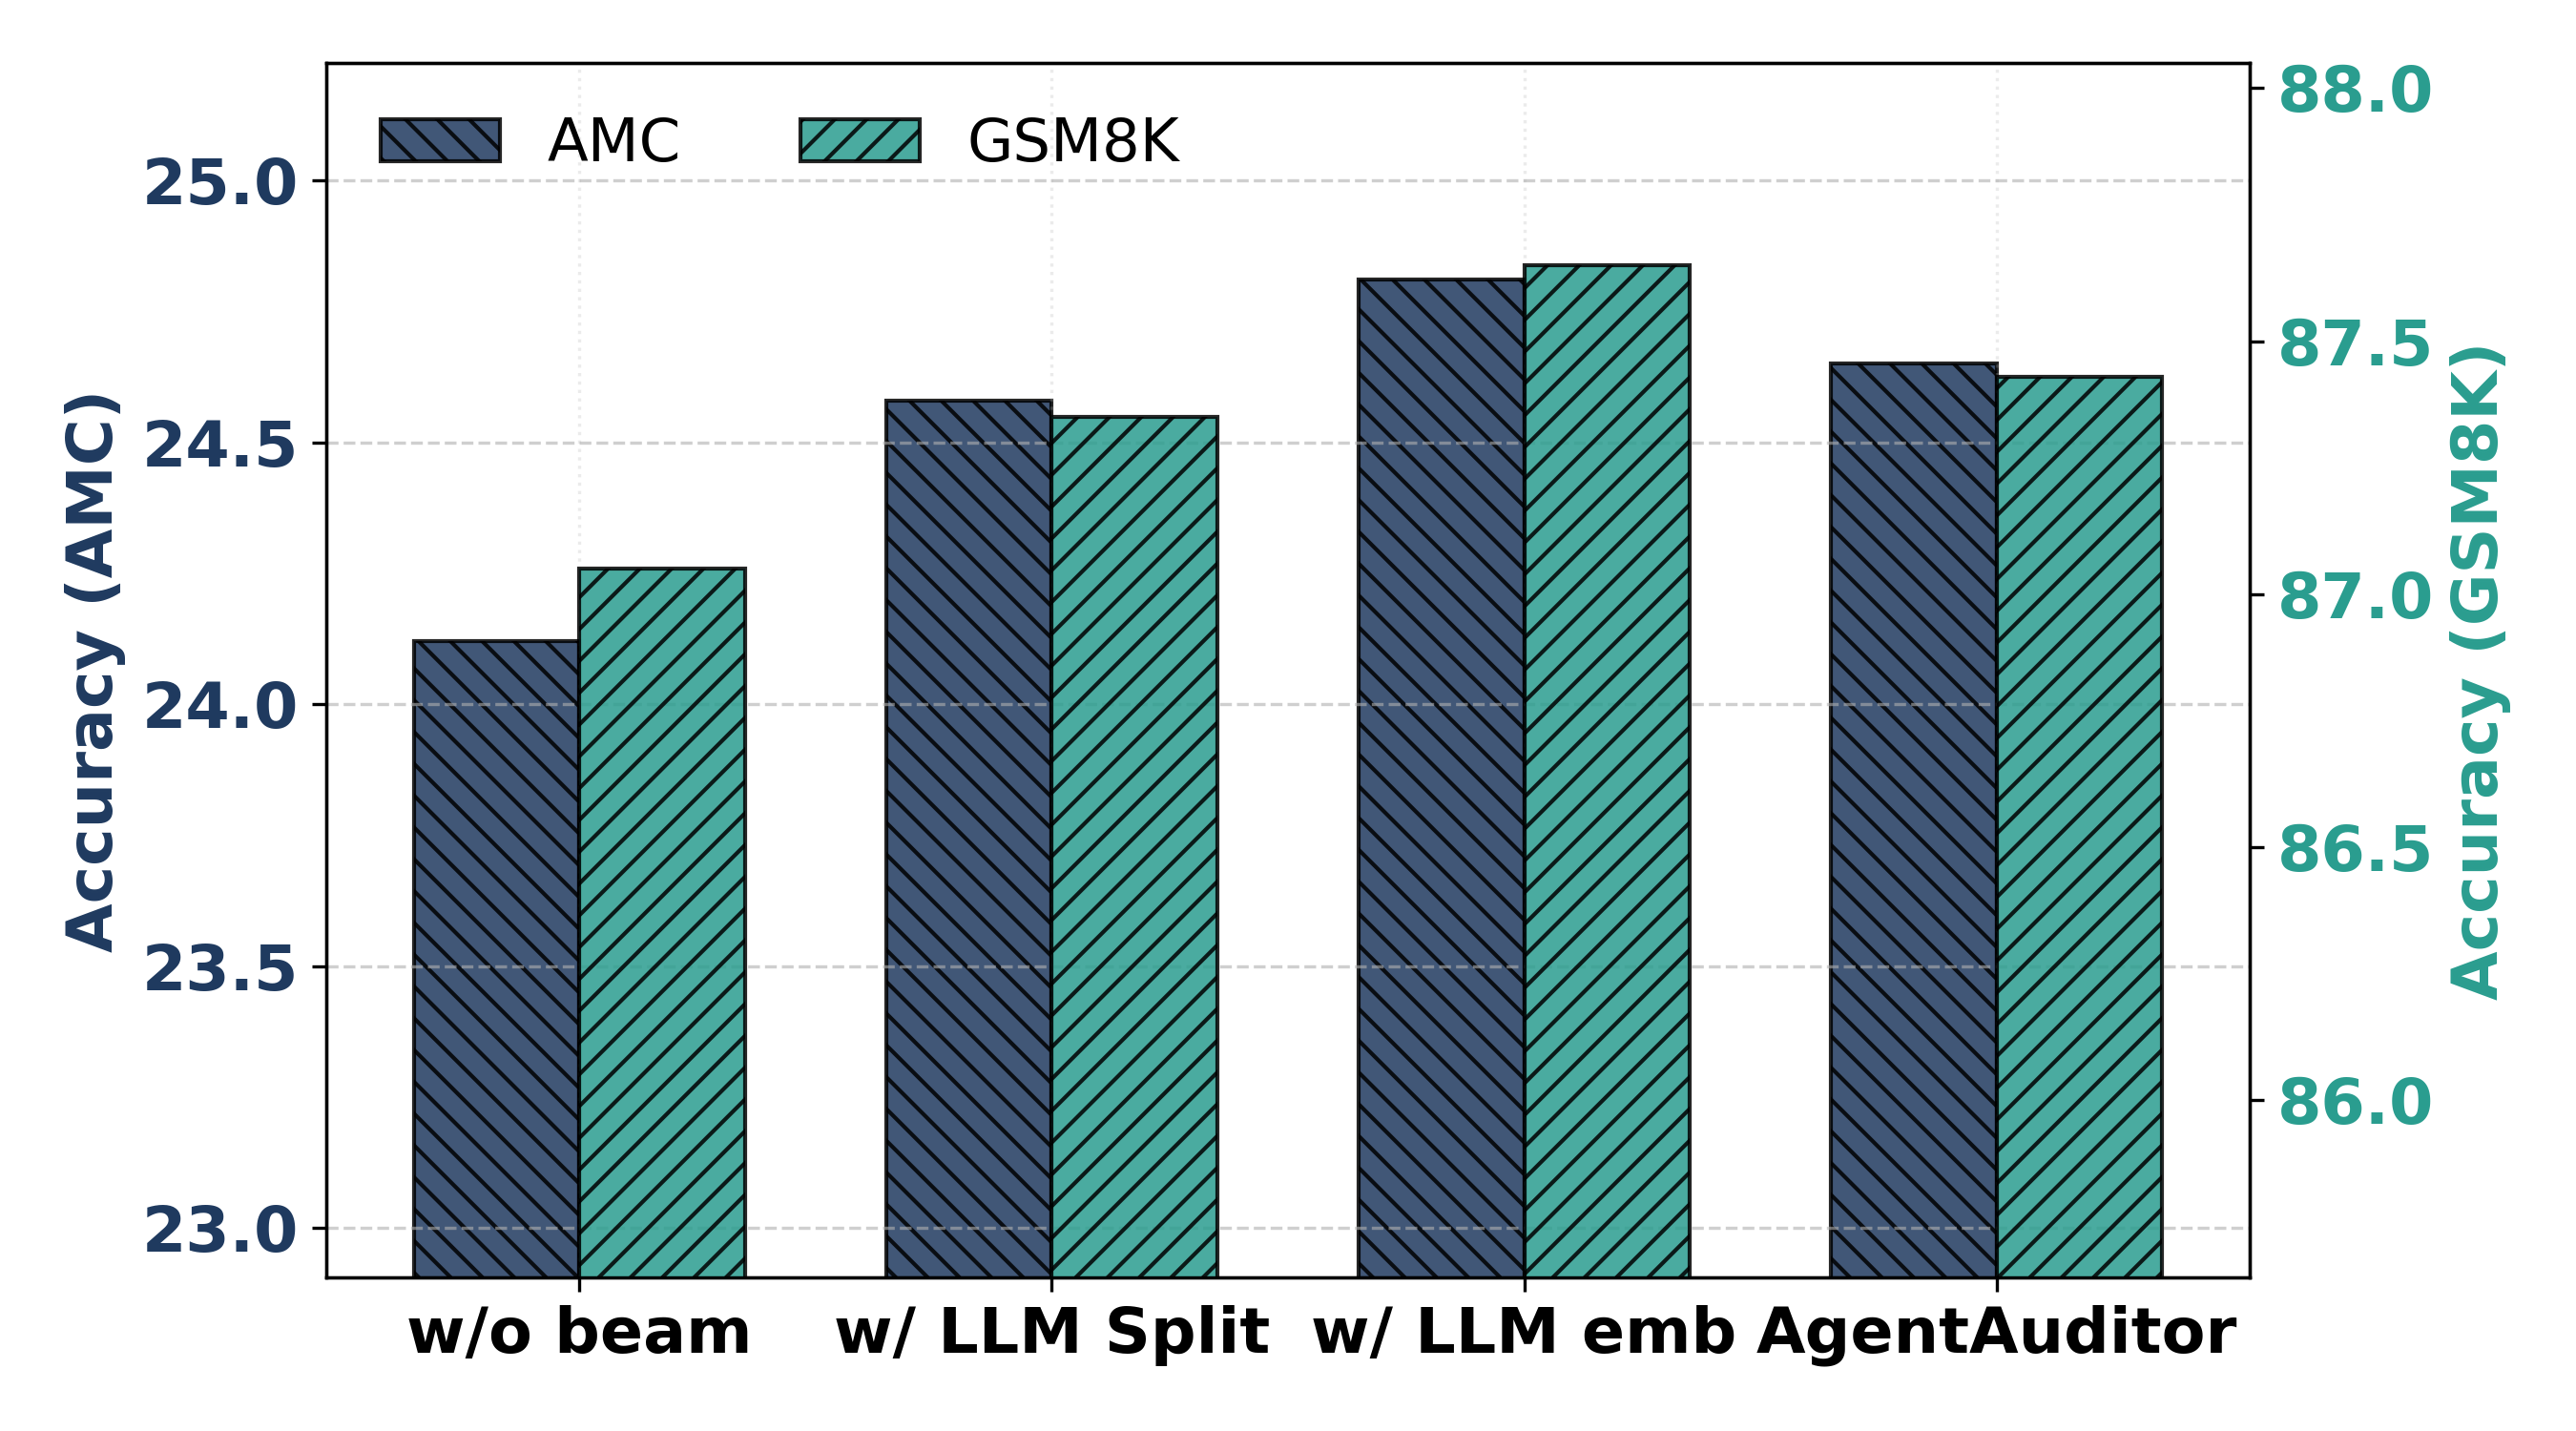
\includegraphics[width=0.9\linewidth]{figures/ablation_beam_split_emb.png}
    \caption{\textbf{Key module ablations for AgentAuditor.} Removing the conditional beam hurts performance, while LLM-based splitting and embeddings yield only minor changes.}
    \label{fig:ab_beam_split_emb}
\end{figure}


\subsection{Analysis: Case Study}

\begin{figure}[t]
    \centering
    
\includegraphics[width=\linewidth]{figures/case_study.pdf}
    \caption{\textbf{Case Study.} Majority Voting fails under confabulation consensus, while \textbf{AgentAuditor} prunes decision-critical divergences by flagging a fatal unit mismatch (mixing cheese/pepperoni across different pizza sizes) and a later constraint violation (spurious ``Kate''), thereby isolating the correct solution.}
    \label{fig:case_study}
\end{figure}

% Figure~\ref{fig:case_study} provides a case study on GSM8K where Majority Voting fails due to confabulation consensus. The diagram illustrates how \textbf{AgentAuditor} identifies and prunes reasoning errors at critical semantic divergence points, such as unit mismatches and constraint violations. This case demonstrates the system's ability to block invalid logic from propagating into a false consensus. For a high-resolution version and detailed step-by-step analysis, please refer to Figure~\ref{fig:case_study_big} and Appendix~\ref{app:case_study}.

Figure~\ref{fig:case_study} provides a case study on GSM8K where Majority Voting fails due to confabulation consensus. The diagram illustrates how AgentAuditor identifies and prunes reasoning errors at critical semantic divergence points. Specifically, the Auditor detects a "fatal unit-mismatch" in Branch 1, where an agent incorrectly combines cheese and pepperoni slices into a single metric that cannot be divided by the differing pizza sizes. Additionally, it filters out a constraint violation in a later step where an agent mistakenly introduces an external entity ("Kate") into the headcount, creating an unnecessary aggregation. By identifying and blocking these invalid branches, AgentAuditor prevents the propagation of flawed logic and isolates the correct solution.


% Figure~\ref{fig:case_study} shows a representative GSM8K example where Majority Voting fails under confabulation consensus, while \textbf{AgentAuditor} succeeds by auditing only decision-critical divergences. All agents start from the same high-level plan (compute slice totals and convert to pies), but the first substantive split appears when one agent prematurely combines cheese and pepperoni slices into a single ``total slices'' quantity. This introduces a unit mismatch. The combined count cannot be mapped consistently to both 12-slice and 8-slice pies. The Auditor flags this at the earliest divergence, selects the branch that preserves per-flavor accounting, and prunes the incompatible aggregation. A second divergence occurs at the slice-to-pie conversion stage. One agent incorrectly adds a ``$\times 7$'' factor by assuming Kate eats the same amount as her friends, even though the problem statement specifies only the friends' consumption. The Auditor again selects the branch that respects the stated constraints and quantities, keeping the conversions well grounded. The final solution follows a clean per-flavor computation (3 cheese pies and 3 pepperoni pies) and yields the correct answer. This case highlights the benefit of structure-aware auditing. By localizing verification to the exact steps where semantics diverge, AgentAuditor blocks early, fluent but invalid transformations from propagating into confident yet incorrect consensus.


\section{Conclusions}
This paper proposes \textbf{AgentAuditor}, an evidence-based adjudication framework that replaces majority voting with structure-aware auditing for multi-agent LLM reasoning. Our findings underscore a shift from popularity-driven aggregation to evidential integrity: across diverse MAS frameworks, benchmarks, and LLM backbones, AgentAuditor consistently improves final decision quality while remaining token-efficient. Future work will focus on tooling-enhanced auditing, integrating external solvers, retrieval, and verification modules to strengthen factual and constraint checking, and more powerful optimization algorithms beyond ACPO to further improve robustness against confabulation consensus and majority-induced bias.


% \newpage


%\section*{Impact Statement}

%This paper proposes an evidence-auditing approach for aggregating multi-agent LLM reasoning under confabulation consensus. The intended benefit is improved reliability in settings where multiple agents are used to support complex problem solving. Our method reduces reliance on vote frequency, which can be misleading under correlated errors, and instead audits branch evidence at decision-critical divergences. This design can help prevent dominant but incorrect consensus outcomes, and it can lower operational cost by avoiding full re-solving when disagreements are localized.

%The work also carries risks that are important to acknowledge. Evidence auditing operates on model-generated traces, so it can inherit hallucinations, omissions, and spurious rationales produced by the agents. A stronger adjudication layer may also increase automation bias, because users can over-trust a system that appears to validate its own reasoning. The method can be misused to make flawed outputs appear more credible, especially when the audited evidence is incomplete or selectively presented. In addition, multi-agent traces may contain sensitive content in practical deployments, so data handling and retention policies matter even when the final answer alone is innocuous.

%These risks can be mitigated with established practices for LLM-based decision support. We recommend evaluation that matches the intended domain, explicit abstention or escalation when the available evidence is insufficient, and targeted monitoring on majority-wrong cases where correlated errors are most likely. Deployments should document how evidence packets are formed and how audit decisions are derived, so outputs are interpreted as support rather than authority. When storing multi-agent traces, privacy-aware logging and access control are necessary. This work improves aggregation for multi-agent reasoning and does not introduce new risk classes beyond typical LLM deployments, though its impact can scale with adoption.




% In the unusual situation where you want a paper to appear in the
% references without citing it in the main text, use \nocite

\bibliography{example_paper}
\bibliographystyle{icml2026}

%%%%%%%%%%%%%%%%%%%%%%%%%%%%%%%%%%%%%%%%%%%%%%%%%%%%%%%%%%%%%%%%%%%%%%%%%%%%%%%
%%%%%%%%%%%%%%%%%%%%%%%%%%%%%%%%%%%%%%%%%%%%%%%%%%%%%%%%%%%%%%%%%%%%%%%%%%%%%%%
% APPENDIX
%%%%%%%%%%%%%%%%%%%%%%%%%%%%%%%%%%%%%%%%%%%%%%%%%%%%%%%%%%%%%%%%%%%%%%%%%%%%%%%
%%%%%%%%%%%%%%%%%%%%%%%%%%%%%%%%%%%%%%%%%%%%%%%%%%%%%%%%%%%%%%%%%%%%%%%%%%%%%%%
\newpage
\appendix
\onecolumn
\section*{Appendix}


\section{Related Work}
\label{app:app_relatedwork}

\subsection{LLM-based Multi-Agent Collaboration for Reasoning}
\label{app:relatedwork_part1}
In recent years, large language models (LLMs) have been widely applied in a variety of practical scenarios~\cite{chen2025tourrank,xia2025hierarchical,zhao2025hierarchical,yang2024enhancing}. Specifically, LLMs have inspired a surge of interest in multi-agent systems (MAS) as a means to extend single-model reasoning capacity~\cite{wu2024autogen,motwani2024malt,ishibashi2024self,yan2025beyond,dai2025multi}. Early frameworks demonstrate that collective interaction among LLMs can mitigate individual cognitive limitations, enabling richer reasoning through distributed exploration and mutual critique~\cite{hong2023metagpt,chen2023agentverse,jiang2023llm,ning2023skeleton,qiao2024autoact,pan2024agentcoord}.  
Existing methods largely fall into two paradigms. \emph{Prestructured collaboration} imposes fixed interaction topologies, such as chains, trees, or debate graphs, to orchestrate discussion and verification~\cite{du2023improving,liu2024groupdebate,qian2024scaling}. These designs enhance coherence but remain bounded by static, human-specified structures that cannot adapt to dynamic task complexity. In contrast, \emph{self-organizing paradigms} dynamically adjust collaboration graphs through routing, pruning, or evolutionary mechanisms, exemplified by frameworks like DyLan, GPTSwarm, and AFLOW~\cite{hu2024automated,shang2024agentsquare,zhang2024cut,zhuge2024gptswarm,zhang2024aflow}.  
While these approaches improve communication efficiency and diversity, most focus on \textit{coordination dynamics} rather than epistemic reliability~\citep{wan2025rema,peiyuan2024agile,feng2024large}. Their optimization is procedural, determining who speaks or when, rather than epistemological, leaving the collective still vulnerable to correlated reasoning errors and unverified consensus~\citep{chen2022ptde,wei2025lero,jiang2025qllm,alsadat2024multi,lin2025speaking}. This limitation motivates the need for a principled adjudication mechanism that evaluates the \textit{content} of reasoning rather than its popularity.

\subsection{Evaluation and Adjudication in Multi-Agent Reasoning}
\label{app:relatedwork_part2}

While multi-agent coordination improves the diversity of reasoning, ensuring the \textit{correctness} of collective outcomes remains a core challenge.  
Early systems aggregate results through \emph{majority voting} or rule-based ensembling~\cite{chan2023chateval,chen2024llmarena,wei2025lero}, assuming that consensus approximates truth.  
In practice, however, agents trained on similar distributions often exhibit \textit{correlated errors}, causing the majority to converge on plausible yet incorrect answers, a phenomenon described as the "tyranny of the majority"~\cite{du2023improving,liu2024groupdebate}. To improve reliability, recent frameworks introduce \emph{referee} or \emph{reviewer} agents that evaluate peers’ reasoning trajectories~\cite{abdelnabi2023llm,du2023improving,zhang2024cut}.  
Debate-style protocols exchange arguments before a third-party judge determines the winner, while \emph{self-consistency} and \emph{peer review} methods aggregate explanations instead of final answers~\cite{chen2023universal,xu2023towards,wang2025mars}.  
Although these approaches enhance reasoning control, they often depend on heuristic templates or task-specific rules rather than a principled notion of evidence and logical soundness.  
Meanwhile, research in \emph{LLM evaluation and verification} explores automatic reasoning validation through reward modeling~\cite{kwon2023reward,lambert2024rewardbench,setlur2024rewarding} and reflective self-evaluation~\cite{xie2023self,zhang2024self,yan2024mirror}, yet these methods focus on single-agent reflection rather than distributed adjudication across agents.  


% \section{Appendix}



% This is an appendix.



\section{Experiments}

\subsection{Experimental Setup}
\label{ref:app_exp_setup}
\paragraph{Tasks and Datasets.}
We evaluate our framework on four representative reasoning benchmarks that collectively assess both domain-specific and general reasoning abilities of large language model (LLM) agents.
\textbf{GSM8K} focuses on grade-school mathematical reasoning through structured word problems.
\textbf{MATH} and \textbf{AMC} provide competition-level problems requiring multi-step symbolic reasoning and algebraic manipulation.
To measure general reasoning competence, we further include the \textbf{MMLU} benchmark, which spans 57 academic and professional domains.
For all datasets~\cite{cobbe2021training,hendrycks2020measuring}, we follow the official evaluation splits and report the standard metrics:
\emph{Solve Rate} for GSM8K, MATH, and AMC, and \emph{Accuracy} for MMLU.

\paragraph{Baselines.}
We compare our framework, \textbf{AgentAuditor}, against a comprehensive suite of single- and multi-agent reasoning paradigms.
Single-agent baselines include the \textit{Vanilla} prompting strategy, \textit{Chain-of-Thought} (CoT)~\cite{wei2022chain}, and \textit{Self-Consistency} (SC)~\cite{wang2022self}.
Multi-agent frameworks encompass debate-based and collaborative systems such as \textit{LLM-Debate}, \textit{PHP}, and \textit{DyLan}.
We also consider dynamic workflow architectures, including \textit{AgentPrune} and \textit{GPTSwarm}.
To ensure a fair comparison, \textbf{AgentAuditor} is integrated as a plug-in adjudication module that replaces the final voting stage with our evidence-audited selection process, while keeping the upstream candidate generation identical across all methods.



\paragraph{Implementation Details.}
Following common practice, we employ three agents and three rounds of interaction unless otherwise specified.
All models are instantiated from publicly available instruction-tuned checkpoints, including
Llama-3.1-8B-Instruct, Llama-3.2-3B-Instruct, Qwen2.5-7B-Instruct, and Qwen2.5-3B-Instruct~\cite{dubey2024llama,bai2023qwen}.
Across all settings, we report the mean performance over three random seeds.
To ensure a fair and reproducible comparison, we keep the overall experimental pipeline aligned with the baselines,
including identical evaluation protocols and consistent prompt formatting.
Unless explicitly noted, the AgentAuditor module shares the same backbone family as the generator agents and does not require
additional supervised training beyond the preference optimization applied in our method variants.

For generation, we adopt nucleus sampling (top-$p$) with $p=0.95$. We use a default decoding temperature of $0.7$ to encourage non-trivial diversity while maintaining stability of final answers.
For training, we apply parameter-efficient fine-tuning via LoRA, using rank $r=16$, scaling factor $\alpha=32$, and dropout $0.05$.
We tune the learning rate over $\{1\times 10^{-5}, 5\times 10^{-5}, 1\times 10^{-4}, 5\times 10^{-4}\}$ and select the best value
based on validation performance under the same selection criterion used for baselines.
We additionally sweep the number of training epochs in the range of 1--3 to avoid overfitting on preference pairs and to maintain
comparable training budgets across methods.
All training experiments are run on 8 NVIDIA A100 GPUs, and we fix all remaining optimization and infrastructure settings to match the corresponding baseline configurations as closely as possible.



% ==========================================
% Appendix: Toy Analysis (2 propositions)
% ==========================================
\section{Theoretical Analysis: Why Voting Fails Under Correlated Errors and Why Structure Helps}
\label{app:toy_analysis}

This section provides a \emph{supporting} theoretical perspective on the failure mode we target.
Our goal is not to introduce a new theory or claim novel guarantees for arbitrary LLM behaviors.
Instead, we use a simple analytical lens to explain (i) why majority voting can fail when agent errors are correlated, leading to
confabulation consensus, and (ii) why structural semantic deduplication followed by localized auditing helps mitigate this issue.
The analysis should be read as an interpretation of the underlying mechanism rather than a complete characterization of all possible deployments.

\subsection{A.1 Majority Voting Under Correlated Correctness}

Let $X_i\in\{0,1\}$ be the correctness indicator from Eq.~\eqref{eq:Xi}, with $\mathbb{P}(X_i=1)=p$ for all $i$.
Define the sample mean $\bar{X}=\frac{1}{N}\sum_{i=1}^N X_i$ and let $\rho$ denote the average pairwise correlation in Eq.~\eqref{eq:rho}.
A common correlated-voting model (e.g., \citealp{austen1996information}) yields
\begin{equation}
\label{eq:var_barX}
\mathrm{Var}(\bar{X})
\;=\;
\frac{p(1-p)}{N}\,\Big(1+(N-1)\rho\Big).
\end{equation}

\begin{proposition}[Failure of independence assumption]
\label{prop:mv_correlation}
If $\rho=0$ and $p>1/2$, then $\mathrm{Var}(\bar{X})=O(1/N)$ and $\bar{X}$ concentrates around $p$, recovering the classical CJT intuition.
If $\rho>0$ is bounded away from $0$, then $\mathrm{Var}(\bar{X})$ does not vanish as $N\to\infty$ (it approaches $p(1-p)\rho$),
so increasing the number of agents does not necessarily improve the reliability of a majority vote.
\end{proposition}

\paragraph{Interpretation.}
When errors are correlated, the ensemble behaves like an ``echo chamber'': a shared bias can simultaneously shift many agents toward the same
incorrect answer. Thus, even large $N$ may not rescue majority voting, because the effective number of independent ``votes'' is much smaller than $N$.
This provides a formal motivation for focusing on \emph{correlation-aware} aggregation rather than purely increasing the number of agents.

\subsection{A.2 Structure Tree as Semantic Deduplication and Auditing as Discrimination}

Our method first maps the multiset of raw outputs $\mathcal{O}=\{o_1,\dots,o_N\}$ into a smaller set of \emph{semantic branches}
(e.g., clusters / lineages in a reasoning Tree). Abstractly, define a semantic deduplication operator
\begin{equation}
\label{eq:dedup_operator}
\mathcal{T}:\{o_1,\dots,o_N\}\;\mapsto\;\{B_1,\dots,B_K\}, \qquad K\ll N,
\end{equation}
where each branch $B_k$ represents a distinct reasoning trajectory and may be supported by multiple agents.
In a confabulation-consensus regime, many agents produce redundant variants of the same erroneous trajectory;
semantic deduplication collapses these redundant hallucinations into (approximately) a single representative branch $B_{\mathrm{err}}$,
preventing frequency alone from dominating the final decision.

After deduplication, the final decision reduces to an evidence-based comparison among a small number of competing branches.
For intuition, consider a simplified two-branch case with one correct branch $B_{\mathrm{cor}}$ and one erroneous consensus branch $B_{\mathrm{err}}$.
Let an auditor choose between them based on the divergence packet (context + branch-specific evidence).
Define the auditor's \emph{discrimination accuracy}
\begin{equation}
\label{eq:q_def}
q \;=\; \mathbb{P}\!\left(\text{Auditor selects } B_{\mathrm{cor}} \;\middle|\; B_{\mathrm{cor}},B_{\mathrm{err}}\right).
\end{equation}

\begin{proposition}[Deduplication removes the ``quantity advantage'']
\label{prop:dedup_pairwise}
Suppose the MAS produces $n_{\mathrm{err}}$ redundant outputs supporting the same erroneous branch $B_{\mathrm{err}}$ and
$n_{\mathrm{cor}}$ outputs supporting the correct branch $B_{\mathrm{cor}}$, with $n_{\mathrm{err}} > n_{\mathrm{cor}}$ (confabulation consensus).
Then majority voting in Eq.~\eqref{eq:mv} selects $y_{\mathrm{err}}$ with probability $1$ under perfect answer extraction.
In contrast, after semantic deduplication that collapses redundant outputs, the aggregation reduces to a small-arity branch comparison; in the
two-branch toy case, the probability of selecting the correct branch is $q$ from Eq.~\eqref{eq:q_def}.
Hence, whenever $q>1/2$, auditing is strictly better than random guessing and can outperform MV on consensus-error instances.
\end{proposition}

\paragraph{Interpretation.}
The key shift is from a \emph{frequency-weighted} decision (``how many agents said this?'') to a \emph{validity-sensitive} decision
(``which branch is better supported by evidence and logic?'').
Semantic tree reduces the decision space from $N$ potentially redundant outputs to $K$ distinct hypotheses, and auditing learns to
discriminate among these hypotheses. This explains why our approach is particularly effective on hard subsets where correlated errors
inflate the apparent support of a wrong answer.

\paragraph{Connection to training.}
Our ACPO objective explicitly trains the auditor on \emph{majority-failure} (trap) instances, where the incorrect branch has higher support
but the correct branch exists. This directly increases the discrimination accuracy $q$ in Eq.~\eqref{eq:q_def} under the confabulation-consensus regime,
aligning optimization with the failure mode described above.





\section{Method}

% =========================
% Section 3.1 (Formal Setup)
% =========================
\subsection{Problem Formulation}
\label{app:formal_setup}

We study answer aggregation for a single query (problem) $q$ with a unique ground-truth answer $y^\star$.
A multi-agent system (MAS) instantiates $N$ agents $\mathcal{A}=\{a_1,\dots,a_N\}$ and produces a set of candidate outputs
$\mathcal{O}=\{o_1,\dots,o_N\}$, where each $o_i$ contains an agent's reasoning trace and a final answer.
Let $\hat{y}(o_i)$ denote the final answer extracted from $o_i$.

\paragraph{Majority voting.}
A standard aggregator is majority voting (MV),
\begin{equation}
\label{eq:mv}
\hat{y}_{\mathrm{MV}}
\;=\;
\arg\max_{y}\; \sum_{i=1}^N \mathbb{I}\big[\hat{y}(o_i)=y\big],
\end{equation}
which estimates the mode of the empirical answer distribution.
Under the classical Condorcet Jury Theorem (CJT), if each agent is correct with probability $p>1/2$ and the correctness
events are independent, then $\mathbb{P}(\hat{y}_{\mathrm{MV}}=y^\star)\to 1$ as $N\to\infty$.

\paragraph{Confabulation consensus (correlated errors).}
In LLM-based MAS, agent errors can be highly correlated due to shared pretraining, prompt anchoring, and interaction dynamics,
leading to \emph{confabulation consensus}: many agents converge to the same (but incorrect) answer with similar reasoning patterns.
To formalize this regime, define the correctness indicator
\begin{equation}
\label{eq:Xi}
X_i \;=\; \mathbb{I}\big[\hat{y}(o_i)=y^\star\big], \qquad i\in\{1,\dots,N\},
\end{equation}
and the average pairwise correlation
\begin{equation}
\label{eq:rho}
\rho \;=\; \frac{2}{N(N-1)}\sum_{1\le i<j\le N}\mathrm{Corr}(X_i,X_j).
\end{equation}
We refer to \emph{hard} instances as those for which $\rho$ is non-negligible (often $\rho>0$), violating the independence
assumption in CJT. Equivalently, one can view correlated errors as arising from a latent ``bias'' variable $Z$ that, when activated,
increases the probability that many agents produce the same incorrect answer $y_{\mathrm{err}}\neq y^\star$:
\begin{equation}
\label{eq:latent_bias}
Z\sim \mathrm{Bernoulli}(\pi), \qquad
\mathbb{P}\big(\hat{y}(o_i)=y_{\mathrm{err}} \,\big|\, Z=1\big) \gg
\mathbb{P}\big(\hat{y}(o_i)=y_{\mathrm{err}} \,\big|\, Z=0\big).
\end{equation}
In this regime, MV can be dominated by the multiplicity of a shared error mode, i.e., $\hat{y}_{\mathrm{MV}}=y_{\mathrm{err}}$ even when
a minority of agents output $y^\star$.

\paragraph{Goal.}
We seek an aggregation procedure $f$ that maps a set of candidate outputs $\mathcal{O}$ to a single final prediction $\hat{y}$,
\begin{equation}
\hat{y} \;=\; f(\mathcal{O},q),
\end{equation}
such that it is (i) \emph{robust to quantity}: it does not automatically privilege an answer solely because it appears many times,
and (ii) \emph{sensitive to validity}: it can recover $y^\star$ when the correct reasoning exists but is outnumbered by correlated errors.
Our method operationalizes this goal by (a) \emph{structural semantic deduplication} of redundant reasoning and (b) \emph{auditing}
at critical divergence points, replacing frequency-based aggregation with evidence-based discrimination.




\subsection{Structure-Adaptive Evidence Auditing}
\label{app:auditing}

While the Reasoning Tree organizes the collective epistemic state, the core of \textbf{AgentAuditor} lies in its adjudication mechanism. Unlike traditional methods that evaluate entire traces in isolation, our framework performs \textit{structure-adaptive auditing}. This process converts the intractable problem of global correctness assessment into a sequence of tractable, local differential diagnoses at specific \textit{Critical Divergence Points (CDPs)}.

\subsubsection{Divergence Diagnosis and Packet Construction}
\label{sec:packet_app}

We traverse the tree $\mathcal{F}$ from the root. A node $u$ is a \emph{Critical Divergence Point (CDP)} if it has at least two outgoing branches, i.e., $|\mathcal{C}(u)| \geq 2$. Such a node marks a rupture in semantic agreement. To provide the Auditor with appropriate context while keeping inputs compact, we characterize the divergence by the \emph{epistemic depth} $d(u)$ (the hop distance from the root) relative to a threshold $\delta$. Intuitively, early branching ($d(u) < \delta$) often corresponds to heterogeneous solution strategies, whereas late branching ($d(u)\geq \delta$) typically indicates localized execution errors within a largely shared approach. We encode this diagnosis as a discrete tag $\text{Type}(u)$ used to condition packet construction.

For each CDP $u$, we build a \emph{Divergence Packet} $\Psi_u$ that consists of (i) the shared prefix history up to $u$ and (ii) compact, branch-specific evidence immediately following the divergence. Let $H_u$ denote the ordered sequence of representative steps along the unique path from the root to $u$. For each child branch $v\in\mathcal{C}(u)$, we extract an evidence segment $E_v$ by taking the next steps along that branch, truncated to a window size $k$ or earlier if another CDP is encountered. The resulting packet is
\begin{equation}
    \Psi_u = \Big\langle \text{Type}(u),\; H_u,\; \{(E_v,\mathcal{S}_v)\mid v\in\mathcal{C}(u)\}\Big\rangle,
\end{equation}
where $\mathcal{S}_v$ is the support set of branch $v$ provided as a heuristic hint (not a decision rule). By isolating $E_v$ and conditioning on $\text{Type}(u)$, we encourage the Auditor to judge the \emph{immediate logical consequence} of the divergence under the shared context $H_u$, rather than being distracted by downstream hallucinations or verbose but irrelevant continuations.


\subsubsection{Context-Aware Adjudication}
\label{sec:adjudication_app}

Unlike generic ``LLM-as-a-Judge'' setups that score isolated outputs, our Auditor adjudicates \emph{within the logical lineage of the dispute}. We instantiate adjudication as a discriminative function $f_{\theta}$ that takes a divergence packet $\Psi_u$ (Sec.~\ref{sec:packet_app}) and selects the most reliable outgoing branch based on contextual evidence.

\paragraph{Auditing input and rubrics.}
For a CDP $u$, the divergence packet $\Psi_u$ explicitly couples the shared prefix history $H_u$ with branch-specific evidence segments $\{E_v\}_{v\in\mathcal{C}(u)}$ and their support hints $\{\mathcal{S}_v\}$. The Auditor evaluates candidate branches under a structured rubric $\mathcal{R}$ consisting of three complementary criteria:
\begin{itemize}
    \item \textbf{Factual Accuracy} ($\mathcal{R}_{\textsc{fact}}$): verifying arithmetic, stated facts, and externally checkable claims;
    \item \textbf{Logical Soundness} ($\mathcal{R}_{\textsc{log}}$): checking deductive validity and consistency with the antecedent context $H_u$;
    \item \textbf{Constraint Adherence} ($\mathcal{R}_{\textsc{con}}$): enforcing problem-specific constraints (e.g., integrality, bounds, or domain conditions).
\end{itemize}
Crucially, $\mathcal{R}$ is applied \emph{contextually}: depending on $\text{Type}(u)$, the Auditor may prioritize factual checks for late-stage computational discrepancies, or emphasize logical/constraint checks for early-stage methodological splits.

\paragraph{Discriminative Output and Rationale.}
The Auditor operates in a \textit{discriminative mode}, outputting a selection decision over the candidate branches $\mathcal{B}$. Formally, given the packet $\Psi_u$, the Auditor predicts the optimal branch $v^*$, a confidence score $\alpha \in [0,1]$, and a natural language justification:
\begin{equation}
    (v^*, \alpha, \text{Rationale}) = f_{\theta}(\Psi_u; \mathcal{R})
\end{equation}
This design effectively decouples the generation capability from the verification capability. Even if the Auditor model lacks the capacity to solve the complex problem from scratch ($P(y|q)$ is low), it can effectively adjudicate between conflicting solutions by leveraging the \textit{comparative hardness principle}: it is epistemically easier to identify the flaw in a localized comparison than to generate a perfect proof \textit{ex nihilo}.


\subsubsection{Recursive Adjudication Process}
The auditing process proceeds as an iterative directed traversal on the tree. Starting from the root, whenever the current node is a CDP $u$, the system invokes the Auditor and obtains a branch preference together with an audit signal $\alpha$. If the Auditor returns a decisive preference, the system commits to the selected branch and prunes the alternatives; otherwise, it defers commitment and invokes the adaptive inference strategy in Sec.~\ref{sec:inference}. In practice, this commit--defer behavior is governed by a configurable trigger $\lambda$ applied to $\alpha$, which we treat as an internal control knob rather than a calibrated probability.


\subsection{Adaptive Inference via Conditional Beam Search}
\label{app:inference}

While structure-adaptive auditing (Sec.~\ref{sec:auditing}) provides a strong local discriminator, strictly committing to a greedy path can incur irreversible error propagation if a single critical adjudication is mistaken. To improve robustness without paying the cost of exhaustive search, we adopt an \textit{adaptive inference strategy} that modulates the search width through a lightweight, policy-controlled commit--defer switch.

We implement a conditional transition rule that defaults to computational economy, but activates a safety valve when the current divergence is deemed ambiguous by the system policy.
At a divergence point $u$, the Auditor selects a provisional winner branch $v^*$ and returns an audit signal $\alpha$ (a coarse indicator of decisiveness). We introduce a system-level trigger $\lambda$ that governs whether the system commits immediately or defers commitment via beam search. The traversal policy $\pi$ is defined as:
\begin{equation}
    \pi(u) = 
    \begin{cases} 
    \textbf{Greedy Mode:} \quad \quad \quad \quad\text{if } \alpha \geq \lambda \\
    \text{Commit to } v^* \text{ and prune branches.} & \\[4pt]
    \textbf{Exploratory Mode:} \quad \quad \text{if } \alpha < \lambda \\
    \text{Activate beam search.} &
    \end{cases}
\end{equation}
Importantly, $\lambda$ is treated as an operator-defined control parameter and $\alpha$ is used only to gate exploration; we do not assume $\alpha$ to be a calibrated probability.

In \textbf{Greedy Mode}, the system performs a deterministic single-path traversal, maximizing efficiency by immediately pruning alternatives at $u$.
In \textbf{Exploratory Mode}, the system maintains an active beam $\mathcal{B}$ of size $K$, allowing multiple competing branches to progress until additional downstream evidence resolves the ambiguity.

\paragraph{Terminal Validation and Consensus Reconciliation}
When exploratory search terminates, the system retains a set of candidate solution lineages $\mathcal{B}_{\text{final}}$.
Rather than relying on mechanical aggregation of local heuristics, we perform a terminal review to synthesize the final decision: we construct a \textit{Consensus Review Packet} that aggregates the full reasoning traces of all surviving candidates, and invoke the Auditor for a direct multi-way comparison over complete chains. This terminal validation acts as a global consistency check, ensuring that the final output is selected based on end-to-end reasoning integrity rather than merely surviving step-wise filtering.





\section{Anti-Consensus Preference Optimization}
\label{app:training}

While the structure-adaptive auditing (Sec.~\ref{sec:methodology}) provides a structural mechanism for resolving disagreements, the Auditor must be trained to remain evidence-driven under misleading social signals. In multi-agent settings, instruction-tuned LLMs often exhibit \emph{sycophancy}: they over-weight majority support or verbosity even when it conflicts with factual or logical validity. To mitigate this \emph{majority trap}, we propose \textbf{Anti-Consensus Preference Optimization (ACPO)}, which constructs preference pairs \emph{specifically} from historical cases where majority voting fails, encouraging the Auditor to learn that \emph{validity is independent of frequency}.

\subsection{The Sycophancy Challenge in Adjudication}
In multi-agent adjudication, majority support becomes a strong contextual prior. Given a divergence packet $\Psi_u$ containing competing branches with different support sizes (e.g., $|\mathcal{S}_{maj}| \gg |\mathcal{S}_{min}|$), an instruction-tuned Auditor tends to favor the majority branch even when it is incorrect. We characterize this tendency as a \textit{sycophancy bias}:
\begin{equation}
\begin{aligned}
    P_{\pi_{\mathrm{ref}}}\!\left(y_{maj}\mid \Psi_u\right)
    \;>\;
    P_{\pi_{\mathrm{ref}}}\!\left(y_{min}\mid \Psi_u\right), \\
    \text{even when } y_{maj} \neq y^\star
\end{aligned}
\end{equation}
where $y^\star$ denotes the ground-truth answer when available. Standard RLHF style training or generic DPO often under-corrects this bias because the resulting preference data are dominated by \emph{majority-correct} cases, which implicitly reinforce the shortcut heuristic that more support implies higher validity. 


\subsection{Constructing the ``Consensus Trap'' Dataset}
To counter the majority-induced prior, we curate a targeted dataset $\mathcal{D}_{\mathrm{trap}}$ from \emph{majority-vote failure} cases. The key idea is to train the Auditor under precisely the conditions where ``support'' is a misleading signal, and to localize supervision to the topological juncture that \emph{separates} the correct minority from the incorrect majority.

\paragraph{Step 1: Majority-failure filtering.}
From a corpus of multi-agent traces with ground truth $y^\star$, we retain instances that satisfy:
(i) the majority answer is incorrect ($y_{\mathrm{maj}} \neq y^\star$), and
(ii) at least one agent produces the correct answer ($\exists\, a_i:\; y_i = y^\star$).
This yields the subset where Majority Vote is provably unreliable by construction.

\paragraph{Step 2: Topological trap localization.}
For each retained instance, we build its Reasoning Tree and identify the \emph{First Point of Disagreement (FPD)} node $u$, i.e., the earliest node at which paths leading to $y^\star$ diverge from paths leading to $y_{\mathrm{maj}}$.
Let $b_{\mathrm{gt}}$ denote the child branch consistent with $y^\star$ (minority-correct) and $b_{\mathrm{err}}$ denote the child branch consistent with $y_{\mathrm{maj}}$ (majority-wrong).
We then extract a \emph{hard} divergence packet $\Psi_{\mathrm{hard}}$ at $u$ (shared context plus short branch evidence), and \emph{include} the support statistics so that the input explicitly contains the misleading social-proof cue (typically $|\mathcal{S}_{b_{\mathrm{err}}}| > |\mathcal{S}_{b_{\mathrm{gt}}}|$).

\paragraph{Step 3: Preference Pairing.}
We formulate the training data as triplets $(x, y_w, y_l)$, where:
\begin{itemize}
    \item $x = \Psi_{hard}$ (The context with misleading majority support).
    \item $y_w$ (Winning) = The adjudication rationale and decision favoring the \textbf{minority} correct branch $b_{gt}$.
    \item $y_l$ (Losing) = The decision favoring the \textbf{majority} incorrect branch $b_{err}$.
\end{itemize}
This construction forces the model to prefer evidence-grounded adjudication over the majority heuristic, because the ``popular'' branch is systematically assigned to the rejected side.


\subsection{Optimization Objective}
We fine-tune the Auditor policy $\pi_{\theta}$ from a fixed reference model $\pi_{\mathrm{ref}}$. 
Given preference triplets $(x, y_w, y_l)\in\mathcal{D}_{\mathrm{trap}}$, ACPO adopts the DPO objective to increase the relative likelihood of the anti-consensus (minority-correct) response $y_w$ over the consensus (majority-wrong) response $y_l$ under the same auditing input $x$:
\begin{equation}
\begin{aligned}
\mathcal{L}_{\text{ACPO}}
= - \mathbb{E}_{\mathcal{D}_{\mathrm{trap}}}\Bigg[&
\log \sigma\!\Bigg(
\beta \log \frac{\pi_{\theta}(y_w \mid x)}{\pi_{\mathrm{ref}}(y_w \mid x)}\\
&-\; \beta \log \frac{\pi_{\theta}(y_l \mid x)}{\pi_{\mathrm{ref}}(y_l \mid x)}
\Bigg)
\Bigg]
.
\end{aligned}
\end{equation}
where $\beta$ controls the strength of the implicit KL regularization to the reference policy. 
Optimizing on $\mathcal{D}_{\mathrm{trap}}$ rather than random pairs directly targets the majority-failure regime, discouraging reliance on support-based heuristics and incentivizing the Auditor to ground its preference in local factual and logical evidence, thereby shifting the decision rule from \textit{popularity-based} to \textit{evidence-based}.



\section{Additinal Results}

\subsection{Case Study}

Figure~\ref{fig:case_study} illustrates a GSM8K example where \emph{Majority Voting} fails due to confabulation consensus, while \textbf{AgentAuditor} succeeds by intervening only at decision-critical semantic divergences. All agents share an apparently consistent macro-plan (compute slice totals, then convert slices to pies). However, this shared prefix hides two qualitatively different error modes that only become salient once we inspect \emph{where} the reasoning topology first forks into incompatible semantic commitments (CDPs). In this instance, two out of three agents reach incorrect answers through different yet locally fluent transformations, so aggregating by final answer amplifies error even when the traces appear coherent at a glance.

\textbf{CDP-1: Type/unit mismatch induced by premature aggregation.}
The first substantive divergence occurs when one agent collapses flavor-specific quantities into a single scalar ``total slices per friend'' (6+4) and proceeds as if this combined count could be converted under both denominators (12 slices per cheese pie and 8 slices per pepperoni pie). This is a latent \emph{type error}: ``cheese-slice'' and ``pepperoni-slice'' are not interchangeable because they belong to distinct conversion regimes. Once merged, the quantity can no longer be mapped consistently back to pie counts without reinstating the per-flavor partition. AgentAuditor identifies this as an early, decisive inconsistency and commits to the branch that preserves flavor-wise accounting (36 cheese slices and 24 pepperoni slices), effectively enforcing a basic invariant for correctness: unit-consistent conversions must be completed before any cross-type summation.

\textbf{CDP-2: Constraint violation via an unsupported multiplicative assumption.}
A later divergence appears during the slice-to-pie conversion stage. Another agent introduces an extra ``$\times 7$'' factor by implicitly including Kate as an additional eater (6 friends + Kate), even though the statement specifies only the friends' consumption. Unlike CDP-1, this is not a conversion/type issue but a \emph{scope/quantifier error} that changes the population being counted. AgentAuditor rejects this branch and selects the alternative that remains grounded in the stated entities and quantities. Importantly, the auditor rationale also favors \emph{trace discipline}: it prefers the branch that performs only necessary transformations and avoids injecting auxiliary assumptions that weaken constraint consistency and are difficult to detect from the final answer alone. This matters in practice because many confabulations arise from seemingly reasonable, statement-ungrounded additions that remain locally plausible and thus can survive naive voting.

\textbf{Why structural tree auditing helps.}
This case highlights how structural tree auditing reshapes the failure surface relative to majority voting. Majority voting operates only on final answers and therefore cannot distinguish between (i) solutions produced by a unit-consistent, statement-grounded pipeline and (ii) solutions produced by fluent but invalid steps that violate a hidden invariant or constraint earlier in the trace. In contrast, the reasoning tree exposes the earliest semantic fork points, allowing the auditor to localize verification to a small number of CDPs rather than re-evaluating entire traces. By pruning branches at the first appearance of irreconcilable unit commitments (CDP-1) or statement-scope violations (CDP-2), AgentAuditor prevents early errors from propagating and being reinforced as confident consensus. The selected path performs clean per-flavor conversions (36/12 and 24/8) and yields the correct purchase count: 3 cheese pies and 3 pepperoni pies, totaling 6.

\begin{figure}[t]
    \centering
    
\includegraphics[width=0.7\linewidth]{figures/case_study.pdf}
    \caption{\textbf{Case Study.} An example where majority voting converges to an incorrect consensus due to correlated fluent errors. AgentAuditor audits only decision-critical divergence points, detects a flavor-unit mismatch and an unsupported population assumption, prunes the invalid branches early, and selects the correct per-flavor conversion path.}
    \label{fig:case_study_big}
\end{figure}


\end{document}

% This document was modified from the file originally made available by
% Pat Langley and Andrea Danyluk for ICML-2K. This version was created
% by Iain Murray in 2018, and modified by Alexandre Bouchard in
% 2019 and 2021 and by Csaba Szepesvari, Gang Niu and Sivan Sabato in 2022.
% Modified again in 2023 and 2024 by Sivan Sabato and Jonathan Scarlett.
% Previous contributors include Dan Roy, Lise Getoor and Tobias
% Scheffer, which was slightly modified from the 2010 version by
% Thorsten Joachims & Johannes Fuernkranz, slightly modified from the
% 2009 version by Kiri Wagstaff and Sam Roweis's 2008 version, which is
% slightly modified from Prasad Tadepalli's 2007 version which is a
% lightly changed version of the previous year's version by Andrew
% Moore, which was in turn edited from those of Kristian Kersting and
% Codrina Lauth. Alex Smola contributed to the algorithmic style files.
